%% Copernicus Publications Manuscript Preparation Template for LaTeX Submissions
%% ---------------------------------
%% This template should be used for copernicus.cls
%% The class file and some style files are bundled in the Copernicus Latex Package, which can be downloaded from the different journal webpages.
%% For further assistance please contact Copernicus Publications at: production@copernicus.org
%% https://publications.copernicus.org/for_authors/manuscript_preparation.html


%% Please use the following documentclass and journal abbreviations for preprints and final revised papers.

%% 2-column papers and preprints
\documentclass[journal abbreviation, manuscript]{copernicus}



%% Journal abbreviations (please use the same for preprints and final revised papers)


% Advances in Geosciences (adgeo)
% Advances in Radio Science (ars)
% Advances in Science and Research (asr)
% Advances in Statistical Climatology, Meteorology and Oceanography (ascmo)
% Aerosol Research (ar)
% Annales Geophysicae (angeo)
% Archives Animal Breeding (aab)
% Atmospheric Chemistry and Physics (acp)
% Atmospheric Measurement Techniques (amt)
% Biogeosciences (bg)
% Climate of the Past (cp)
% DEUQUA Special Publications (deuquasp)
% Earth Surface Dynamics (esurf)
% Earth System Dynamics (esd)
% Earth System Science Data (essd)
% E&G Quaternary Science Journal (egqsj)
% EGUsphere (egusphere) | This is only for EGUsphere preprints submitted without relation to an EGU journal.
% European Journal of Mineralogy (ejm)
% Fossil Record (fr)
% Geochronology (gchron)
% Geographica Helvetica (gh)
% Geoscience Communication (gc)
% Geoscientific Instrumentation, Methods and Data Systems (gi)
% Geoscientific Model Development (gmd)
% History of Geo- and Space Sciences (hgss)
% Hydrology and Earth System Sciences (hess)
% Journal of Bone and Joint Infection (jbji)
% Journal of Micropalaeontology (jm)
% Journal of Sensors and Sensor Systems (jsss)
% Magnetic Resonance (mr)
% Mechanical Sciences (ms)
% Natural Hazards and Earth System Sciences (nhess)
% Nonlinear Processes in Geophysics (npg)
% Ocean Science (os)
% Polarforschung - Journal of the German Society for Polar Research (polf)
% Primate Biology (pb)
% Proceedings of the International Association of Hydrological Sciences (piahs)
% Safety of Nuclear Waste Disposal (sand)
% Scientific Drilling (sd)
% SOIL (soil)
% Solid Earth (se)
% State of the Planet (sp)
% The Cryosphere (tc)
% Weather and Climate Dynamics (wcd)
% Web Ecology (we)
% Wind Energy Science (wes)


%% \usepackage commands included in the copernicus.cls:
%\usepackage[german, english]{babel}
%\usepackage{tabularx}
%\usepackage{cancel}
%\usepackage{multirow}
%\usepackage{supertabular}
%\usepackage{algorithmic}
%\usepackage{algorithm}
%\usepackage{amsthm}
%\usepackage{float}
%\usepackage{subfig}
%\usepackage{rotating}


\begin{document}

\title{Validation of the ALARO1-SFX (CY43T2) regional climate model over Belgium across different resolutions}

% \Author[affil]{given_name}{surname}

\Author[1][wout.dewettinck@ugent.be]{Wout}{Dewettinck} %% correspondence author
\Author[2]{Hans}{Van de Vyver}
\Author[2]{Daan}{Degrauwe}
\Author[2,3]{Rafiq}{Hamdi}
\Author[2]{Michiel}{Van Ginderachter}
\Author[2,4]{Bert}{Van Schaeybroeck}
\Author[2,4]{Kwinten}{Van Weverberg}
\Author[1,2]{Kobe}{Vandelanotte}
\Author[1,2]{Steven}{Caluwaerts}
\Author[1,2]{Piet}{Termonia}

\affil[1]{Department of Physics and Astronomy, Ghent University (UGent), Ghent, Belgium}
\affil[2]{Royal Meteorological Institute of Belgium (RMIB), Brussels, Belgium}
\affil[3]{Xinjiang Institute of Ecology and Geography, Chinese Academy of Sciences, Urumqi 830011, China}
\affil[4]{Department of Geography, Ghent University (UGent), Ghent, Belgium}

%% The [] brackets identify the author with the corresponding affiliation. 1, 2, 3, etc. should be inserted.

%% If an author is deceased, please mark the respective author name(s) with a dagger, e.g. "\Author[2,$\dag$]{Anton}{Smith}", and add a further "\affil[$\dag$]{deceased, 1 July 2019}".

%% If authors contributed equally, please mark the respective author names with an asterisk, e.g. "\Author[2,*]{Anton}{Smith}" and "\Author[3,*]{Bradley}{Miller}" and add a further affiliation: "\affil[*]{These authors contributed equally to this work.}".


\received{}
\pubdiscuss{} %% only important for two-stage journals
\revised{}
\accepted{}
\published{}

%% These dates will be inserted by Copernicus Publications during the typesetting process.

\runningauthor{TEXT}
\runningtitle{TEXT}

\firstpage{1}

\maketitle

\begin{abstract}
Regional climate modeling is essential for providing reliable information to understand localized impacts and guide adaptation strategies in the context of climate change. This study validates long-term continuous climate simulations over Belgium performed with the ALARO1-SFX model, a novel version of ALARO-1 that incorporates an advanced surface scheme (SURFEX) and improved physiographic datasets.

A scale-selective validation setup is introduced, employing a multi-level dynamical downscaling framework to assess the progressive added value of increasing resolution from the mesoscale to convection-permitting scales. The model's performance is evaluated against a gridded observational dataset and precipitation station measurements, focusing on temperature and precipitation biases, diurnal precipitation cycles, and extreme precipitation statistics.

Results indicate that higher resolutions (12.5 km and 4 km), combined with the integration of SURFEX into ALARO1-SFX, improve temperature and precipitation biases relative to the 25 km simulation, with the 4 km resolution providing the best representation of hourly extreme precipitation and its diurnal cycle. However, all simulations exhibit varying degrees of wet and cold biases. The findings underscore the added value of convection-permitting modelling for resolving extreme precipitation events and improving diurnal precipitation cycles. Furthermore, the study provides experimental evidence that increasing model resolution adds value for simulating extreme precipitation even when employing a scale-aware deep convection parameterization.
\end{abstract}


% \copyrightstatement{TEXT} %% This section is optional and can be used for copyright transfers.


\introduction  %% \introduction[modified heading if necessary]

As climate change intensifies, the demand for reliable and local climate information has become increasingly critical for understanding localized impacts and guiding effective adaptation strategies~\citep{IPCC_AR6_ch12}.
To this end, state-of-the-art global circulation models (GCMs) perform simulations within the latest phase of the Coupled Model Intercomparison Project, CMIP6~\citep{eyring_overview_2016}. 
These models typically run at a horizontal resolution of 50--250 km~\citep{nguyen_selecting_2024, IPCC_AR6_WG1_ANNEX2, IPCC_AR6_ch1}.
At such resolutions, GCM simulations accurately represent large-scale dynamics and responses to external forcings.
However, data at these resolutions are often too coarse for many applications, including local impact models.
Additionally, these models fail to account for certain sub-grid characteristics (e.g., complex topography, land-sea contrasts, or land cover heterogeneities) and mesoscale dynamical processes, such as deep convection~\citep{rummukainen_added_2016, giorgi_thirty_2019, lucas-picher_convection-permitting_2021}.
These processes are included in GCMs through parameterization schemes.
Global model simulations at higher resolutions would alleviate these problems, but these are rendered unfeasible due to the immense computational cost~\citep{fuhrer_near-global_2018}.

Regional climate models (RCMs) address this computational cost by simulating only a limited area instead of the entire globe but at a higher resolution~\citep{giorgi_thirty_2019}.
Thereby, however, lateral boundary conditions need to be provided to RCMs by other datasets. 
These boundary conditions can originate from GCM simulations or from (global) reanalysis data, such as the ERA5 dataset~\citep{hersbach_era5_2020}.
Typically, long-term climate simulations with an RCM employ a resolution of 10--50 km.
Compared to GCM output, this finer-scale output adds value particularly in regions featuring diverse topography and varying land-cover properties~\citep{rummukainen_added_2016, IPCC_AR6_ch10}.
Nevertheless, at such scales, deep convective processes are still parameterized and not explicitly resolved. 
This is a well-known source of model uncertainty for precipitation, evident in e.g., excessive light precipitation and a too early peaking diurnal convective cycle~\citep{ban_evaluation_2014,fosser_benefit_2015, hohenegger_towards_2008, kendon_realism_2012,vergara-temprado_climate_2020}.
However, for climate models with resolutions higher than $\sim 5$ km, these processes are in fact (partially) resolved~\citep{prein_review_2015, lucas-picher_convection-permitting_2021}.
Models operating at these scales are referred to as convection-permitting models (CPMs).

CPMs typically turn off their convective parameterization schemes~\citep{coppola_first--its-kind_2020}.
However, the boundary between convection-permitting and convection-parameterized scales is not well defined.
In the so-called `grey zone of convection' ($\sim 4$-$10$ km), deep convection is only partially resolved, making it unclear whether parameterization is required~\citep{vergara-temprado_climate_2020}.
The development of scale-aware convective parameterization schemes addresses this problem.
Rather than simply switching convection on or off, these schemes adapt to the resolution by adjusting their tuning parameters accordingly.
Therefore, models with these parameterization schemes can operate at both coarse and fine resolutions and even in the grey zone.

CPMs have been shown to improve some notable limitations associated with the low-resolution parameterization of deep convection. 
For instance, they improve the diurnal cycle of precipitation, as demonstrated in studies across Europe, including Belgium~\citep{de_troch_application_2016, brisson_how_2016}, and more widely across the continent~\citep{berthou_pan-european_2020}. 
Furthermore, while RCMs generally underestimate precipitation extremes at sub-daily durations~\citep{berg_summertime_2019}, these extremes are better represented in long-term CPM simulations, as shown by \citet{coppola_first--its-kind_2020} and \citet{fosser_convection-permitting_2024}, and studies over Belgium \citep{de_troch_multiscale_2013, tabari_local_2016, van_de_vyver_evaluation_2021} and the Alpine-Mediterranean region~\citep{muller_evaluation_2023, muller_climate_2024}. 
This improvement in extreme precipitation was also noted in the evaluation of an ensemble of kilometre-scale simulations over Europe and the Mediterranean~\citep{pichelli_first_2021, ban_first_2021, ha_precipitation_2024}. 
While precipitation is often the primary focus of added value studies for CPMs, it has also been found that temperature is better represented due to improved representations of topography, clouds, precipitation, and land cover~\citep{leutwyler_evaluation_2017, lucas-picher_convection-permitting_2021, soares_added_2022}.

Despite these advancements, significant model uncertainties remain, particularly in climate projections. 
These uncertainties are often larger than projection uncertainties in the short term~\citep{lehner_partitioning_2020}.
While increasing resolution tends to reduce these uncertainties, as suggested by~\citet{fosser_convection-permitting_2024}, they remain substantial even in CPMs. 
This is because higher resolution alone is not a panacea; e.g., microphysics processes remain parameterized in CPMs, contributing to significant uncertainties~\citep{prein_review_2015, lucas-picher_convection-permitting_2021}. 
Therefore, it is crucial to maintain model diversity to reliably estimate these uncertainties~\citep{IPCC_AR6_ch10}.
However, the diversity of RCMs is decreasing, as seen in the current iteration of EURO-CORDEX simulations, due to the high community effort required to develop and maintain such models~\citep{jacob_regional_2020, cordex_cmip6_downscaling_plans}.

In this study, we present an updated version of the ALARO-0 regional climate model originally introduced by the~\citet{de_troch_multiscale_2013}, where the surface scheme ISBA is now replaced by the SURFEX (Surface Externalisée) scheme~\citep{hamdi_evaluating_2014}. 
This ALARO model was originally developed for numerical weather prediction (NWP) by the ALADIN consortium\footnote{The ALADIN consortium merged with the HIRLAM consortium in 2020 to form the ACCORD consortium.}, which comprised the national (hydro)meteorological services of 16 European and northern African countries~\citep{termonia_aladin_2018}.
The ALARO model is one of three canonical model configurations (CMCs) within the ALADIN framework, along with the baseline ALADIN model and the AROME model.
For a more detailed description, we refer to~\citet{termonia_aladin_2018} and to Sect. \ref{sect:data_methods}.

The key feature of the ALARO physics package is the 3MT (Modular Multiscale Microphysics and Transport) scheme, which handles convection, turbulence, and microphysics~\citep{gerard_evolution_2005, gerard_integrated_2007, gerard_cloud_2009}.
The 3MT scheme has a unique scale-aware character, so that it can determine itself which processes are resolved at a specific resolution.
This provides a smooth multiscale transition from fully-parameterized mesoscale resolutions over the grey zone to fully convection-resolving scales.
This multi-scale feature of the ALARO model is unique with respect to other convection-permitting models and makes it the ideal candidate for a multi-resolution model validation from the mesoscale up to the convection-permitting scales.
Climate simulations will therefore be validated at three different resolutions in this study.
Validating models at different resolutions is essential for both practical and scientific reasons. 
From a practical perspective, the computational demands of high-resolution simulations, particularly at convection-permitting scales, are prohibitive for many research groups. 
As a result, lower-resolution RCMs remain widely used.
Scientifically, examining how model representation of the climate evolves with changing resolution is crucial for improving our understanding and interpretation of simulation results.

The ALARO model originally used the ISBA (Interaction Soil-Biosphere-Atmosphere) scheme~\citep{noilhan_simple_1989, noilhan_isba_1996} for land-surface parameterization, which simulates energy and water exchanges between the surface and the atmosphere.
The new ALARO1-SFX configuration relies on SURFEX~\citep{masson_surfexv72_2013} in order to extend ISBA’s vegetation-based approach by including multiple surface types: nature, urban areas, lakes, and seas. 
This step is necessary to use ALARO-1 for land use climate studies.

In this study, we evaluated long-term climate simulations with the ALARO-1 model at three different resolutions: 25 km, 12.5 km, and 4 km. 
Previous climate simulations with ALARO-0 have been extensively validated, particularly over Belgium \citep{de_troch_multiscale_2013, hamdi_evaluating_2014, giot_validation_2016, tabari_local_2016, berckmans_reinitialised_2017, top_evaluation_2021}. 
These studies employed ALARO cycle 36, following the versioning system aligned with the cycles of the global IFS and ARPEGE models \citep{termonia_aladin_2018}. 
In contrast, this study utilized a more recent version, ALARO cycle 43t2. 
Moreover, from cycle 40 onwards, ALARO underwent substantial updates, leading to the development of ALARO-1.
This new version marked a step-wise change compared to the original ALARO-0.
It introduced significant advancements, including the ACRANEB2 radiation scheme~\citep{masek_single_2016, geleyn_single_2017} and the TOUCANS scheme~\citep{duran_compact_2014, marquet_general_2013} for turbulence and shallow convection. 
The use of ALARO-1 at higher resolutions in this study marks a novel contribution.
The combination of ALARO-1 with SURFEX v8.0 (as used in this study) will be denoted by ALARO1-SFX.
More generally, the term ALARO-1 will refer to the current version of the ALARO model, irrespective of the surface scheme used. 
The broader term ALARO is used when referring to the model in general or when the specific cycle is clear from the context.

The structure of this paper is as follows. Section \ref{sect:data_methods} provides a discussion of the model and the experimental design. 
Following this, the observational datasets and verification methods used in this study are described in detail. 
Section \ref{sect:results} presents the results of the validation, highlighting the model's performance across different resolutions and comparing it with observational data. 
In Sect. \ref{sect:discussion}, these results are discussed and placed in a broader context, comparing them with those from previous ALARO-simulations.
Finally, Sect. \ref{sect:conclusions} draws the conclusions, summarizing the key findings of the study while addressing the limitations and suggesting directions for future research.


\section{Data \& methods}
\label{sect:data_methods}

\subsection{Model and experimental design}

\subsubsection{ALARO1-SFX model}

Historically, the ALARO model has its roots in the global Integrated Forecast System (IFS) of the ECMWF\footnote{European Centre for Medium-Range Weather Forecasts} and the global ARPEGE\footnote{Action de Recherche Petite Echelle Grande Echelle} model of Météo-France.
These global models were adapted to run on a limited area, which resulted in ALADIN.
The ALADIN model employs the same physical parameterization schemes as the global ARPEGE model.
ALARO is in turn a further development of ALADIN: it  shares the dynamical core of ALADIN, but it contains different physics parameterizations.

The dynamical core of ALARO 
can be run both hydrostatically and non-hydrostatically~\citep{bubnova_integration_1995, termonia_aladin_2018}. 
In both configurations, the dynamical equations are spatially discretized using a spectral representation of double-Fourier modes.
For the time-step algorithm, a semi-implicit semi-Lagrangian scheme is employed. 
In the vertical dimension, the model uses a hybrid terrain-following pressure coordinate~\citep{simmons_energy_1981, laprise_euler_1992}. 

ALARO-1 can be coupled to the land-surface model SURFEX, which considers four types of land surface: nature, urban areas, lakes and seas.
For every grid box, a fraction is defined for each of these four types in a tiling approach.
The interaction with the free atmosphere is then calculated by type-specific schemes: ISBA for nature, TEB for urban areas, WATFLUX for lakes and SEAFLUX for seas.
The separate variables of each tile are finally aggregated with a weighted average to compute grid-box values.

\subsubsection{Experimental design}

Firstly, a simulation was run at a resolution of 25 km (see Fig.~\ref{fig:domains_stations}) with the ALARO-1 model using boundary conditions from the ERA-5 reanalysis dataset~\citep{hersbach_era5_2020}. 
Next, this simulation data was dynamically downscaled to two higher resolutions with a multi-level nesting strategy: each higher-resolution run was coupled hourly to the previous lower-resolution run at the boundaries.
The output of all simulations was stored at an hourly frequency.
This downscaling resulted in simulations at 12.5 km and 4 km coupled to, respectively, the 25 km and 12.5 km simulations. 
Henceforth, we will refer to each simulation as ALARO-$x$km with $x$ the resolution in kilometers. 
For the lateral boundary coupling, the Davies relaxation scheme was employed~\citep{davies_lateral_1976}, with a coupling zone of 8 points~\citep{termonia_aladin_2018}.

All simulations span a period of 32 years from 1 January 1991 to 31 December 2022. 
The first year was discarded for each simulation to ensure the model, specifically the soil, reached an equilibrium state. 
The simulations are continuous, with monthly updates to certain (otherwise) constant fields including the sea surface temperature, the surface roughness length, surface albedo, surface emissivity, and the vegetation parameters. 
This monthly update methodology was also applied in~\citet{giot_validation_2016} and~\citet{top_evaluation_2021}.

The different simulation domains are shown in the top panel of Fig.~\ref{fig:domains_stations}. 
The ALARO-25km and ALARO-12km simulations both cover the EURO-CORDEX domain~\citep{jacob_regional_2020}. 
The ALARO-4km simulation covers a smaller domain due to computational constraints. 
This domain is the operational NWP domain of the Royal Meteorological Institute of Belgium. 
It is centred on Belgium and covers parts of Western Europe. 

\begin{figure}[t]
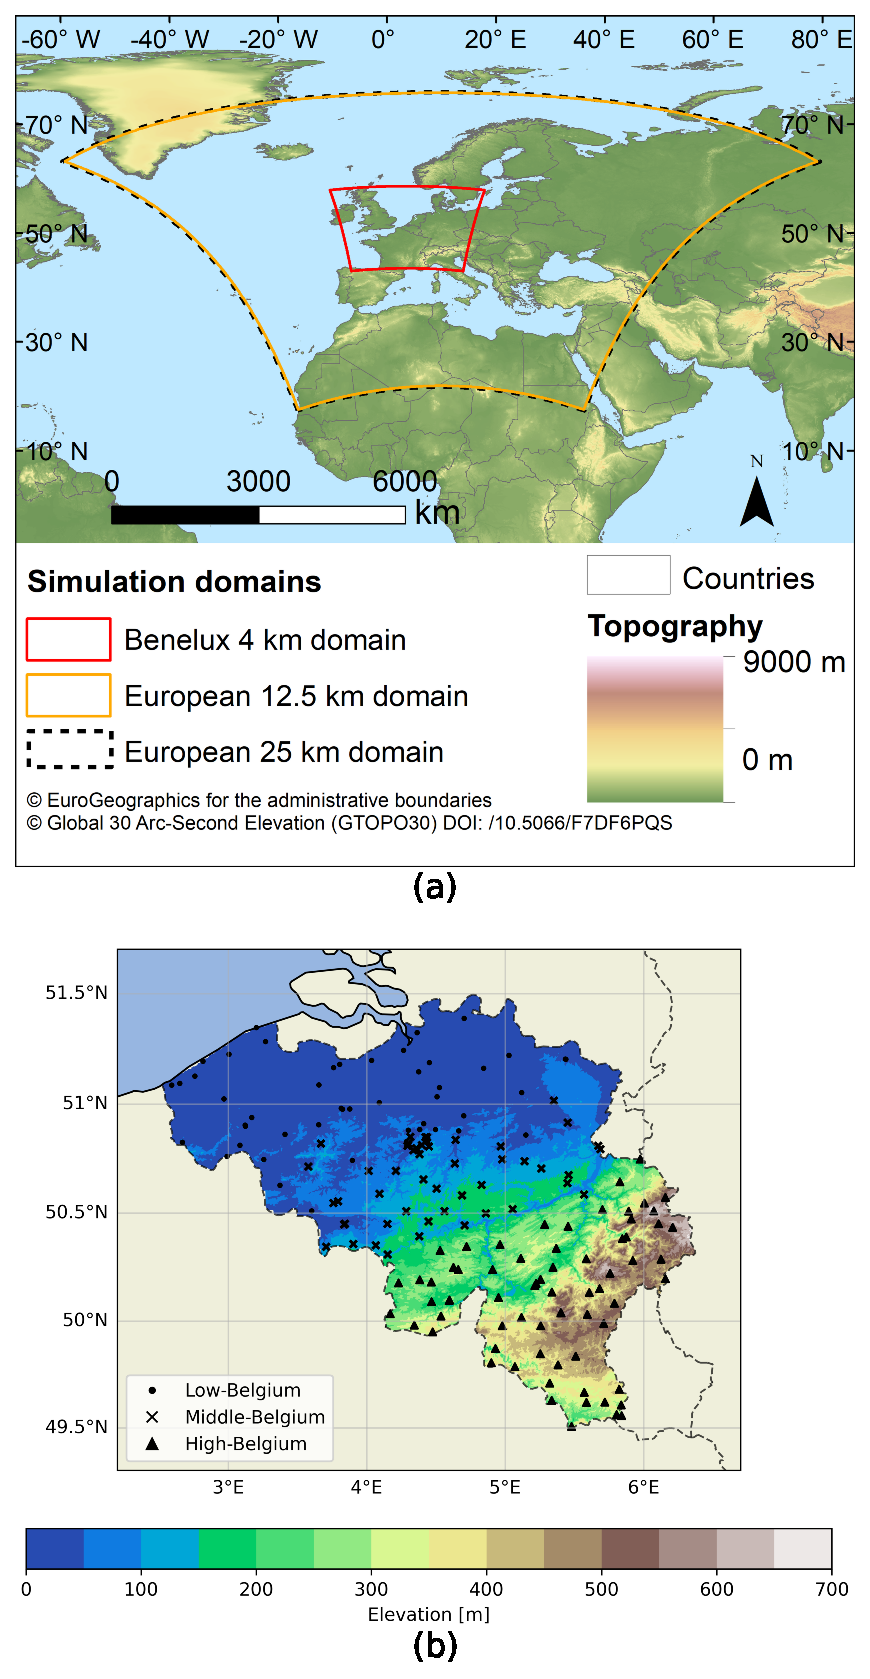
\includegraphics[width=8.3cm]{figures/fig01.pdf}
\caption{(a) Map showing the three simulation domains used in this study, with each domain corresponding to an ALARO-1 simulation at a specific resolution: 25 km, 12.5 km, and 4 km, as indicated in the figure legend. (b) Map of Belgium displaying the elevation above sea level, with precipitation measurement stations marked. The marker styles (circles, squares, and triangles) denote the topographic regions each station is assigned to: Low-Belgium (0--50 m), Middle-Belgium (50--200 m), and High-Belgium (>200 m). ©EuroGeographics and ©GTOPO30}
\label{fig:domains_stations}
\end{figure}

The main technical specifications of the simulations are outlined in Table \ref{tab:technical}. 
All simulations used the hydrostatical dynamical core and are run with 46 vertical levels.
Moreover, they all used the same physics parameterization framework, including the 3MT scheme for deep convection, which adapts to the model resolution due to its scale-aware nature.
One significant difference between the simulations concerns the land-surface scheme. 
SURFEX was not employed for ALARO-25km: instead, the original ISBA scheme was used. 

The main reason for omitting SURFEX in the 25 km simulation is that urban effects are minimal at this resolution, making its inclusion less relevant. 
This setup also aligns more closely with the one used in previous simulations from~\citet{giot_validation_2016}.

%t
\begin{table}[t]
\caption{Technical specifications of simulations with the ALARO-1 model. This table outlines the main differences between each of the three simulations, while the common features are described in the text.}
\begin{tabular}{lccc}
\tophline
Simulation & ALARO-25km & ALARO-12km & ALARO-4km \\
\middlehline
Resolution & 25 km & 12.5 km & 4 km \\
Domain size & 251 x 251 points & 499 x 499 points & 421 x 421 points \\
Time step & 450 s & 300 s & 180 s \\
Lateral boundary coupling & ERA-5 reanalysis & ALARO-25km & ALARO-12km \\
Land surface scheme & ISBA & SURFEX v8.0 & SURFEX v8.0 \\
\bottomhline
\end{tabular}
\belowtable{} \label{tab:technical}
\end{table}

\subsection{Observational data}
\label{sect:obs}

The simulations were validated using the CLIMATE-GRID (CG) dataset, a Belgian 5 km gridded observational dataset based on interpolated station data and developed at the Royal Meteorological Institute of Belgium. 
The dataset spans the period from 1961 until the present day.
It includes daily average temperature and daily total precipitation, which are provided as areal averages over each pixel of the 5 km grid. 

For sub-daily observations of precipitation, we employed station measurements from five measurement networks: VMM in Flanders, DGH in Wallonia, IBGE in Brussels, and the HYDRO and AWS networks covering all of Belgium. 
The VMM and DGH networks are managed by the Vlaamse Milieumaatschappij and the Direction de la Gestion Hydrologique of SPW Mobilité et Infrastructures, respectively. 
The IBGE network, established by the Ministry of the Brussels-Capital Region, has been managed by Brussels Environment since 2007~\citep{dehem2010validation, journee2014validation}. 
The AWS and HYDRO networks are operated by the Royal Meteorological Institute of Belgium~\citep{van_de_vyver_observed_2021}.
The station locations are shown in the bottom panel of Fig.~\ref{fig:domains_stations}, while details about each network are provided in table \ref{tab:stations}.
Rainfall data from all networks were aggregated to an hourly resolution to align with the temporal resolution of the simulation output.

\subsection{Validation metrics and data pre-processing}

The ALARO-1 simulations were evaluated by calculating the mean bias for near-surface air temperature (simply called temperature from here on) and accumulated precipitation depth on annual, seasonal, and monthly timescales. 
For an exact mathematical formulation, we refer to appendix \ref{sect:bias_definition}.

To ensure a consistent comparison, all data were regridded to a common latitude-longitude grid with a spacing of $0.07\degree$ longitude by $0.045\degree$ latitude, which closely aligns with the 5 km resolution of the CG dataset. 
For precipitation, a conservative remapping was applied to all simulations to preserve the spatially averaged precipitation depth~\citep{jones_first-_1999}. 
For temperature, the same conservative procedure was used to reproject ALARO-4km. 
For ALARO-12km and ALARO-25km, another regridding method was employed for temperature.
Since low-resolution data were interpolated to a higher resolution, a conservative regridding method would effectively function as a nearest-neighbor approach in such cases.
Therefore, a bilinear interpolation procedure was used instead, as it was more suitable for the smooth nature of temperature fields.

\subsection{Definition of extreme precipitation}
\label{sect:methods extreme precipitation}

Simulations at convection-permitting scales generally add value through the improved representation of convection and, consequently, of precipitation in general. 
Therefore, this validation study also focused on the statistics of extreme precipitation over Belgium. 
Extreme precipitation events were here defined as the annual maximum (AM) value for a given duration at a specific location or grid point. 
An advantage of this definition is its simplicity: there is no need to determine an arbitrary threshold. 
AM values were selected for durations of 1, 2, 3, 6, 12, 24, 48, and 72 hours using a rolling-window approach over the hourly precipitation data. 

The statistics of these AM values were calculated by fitting a generalized extreme value (GEV) distribution, as defined in eqs. (\ref{eq:GEV}) - (\ref{eq:GEV0})~\citep{coles_introduction_2001}. 
A GEV distribution is defined by three parameters: the shape $\xi$, location $\mu$, and scale $\sigma$. 
These parameters were fitted for each duration separately with the L-moments method as defined by~\cite{hosking_l-moments_1990}. 
Consequently, these parameters were used to calculate the $T$-year return level of $d$-hourly precipitation intensity $z_d(T)$. 
For a mathematical description, we refer to appendix~\ref{sect:gev_definition}.

Next, we applied the regional frequency analysis framework (RFA), as introduced by~\citet{hosking_statistics_1993}. 
The idea behind this framework is to aggregate rainfall data from different locations that share the (presumably) identical underlying distribution. 
A single fitting procedure is then performed for an entire region instead of fitting a separate distribution in each point, allowing for a more robust fit. 
Note that the rainfall data were aggregated and not averaged over a region.
Recent literature, such as the work by~\citet{carreau_partitioning_2017} and~\citet{guerreiro_unravelling_2024}, further supports the use of RFA for improving precipitation extreme estimations. 

We subdivided Belgium into three distinct regions based on elevation: Low-Belgium (0--50 m), Middle-Belgium (50--200 m) and High-Belgium (> 200 m), as shown in Fig.~\ref{fig:domains_stations}. Elevation was used as a discriminatory parameter since it correlates strongly with the annual precipitation totals, which themselves are closely linked to precipitation extremes~\citep{van_de_vyver_spatial_2012}. 
This subdivision strikes a balance between reducing uncertainties and maintaining relatively homogeneous climatic conditions within each region, as suggested by~\citet{van_de_vyver_spatial_2012}.

The return levels for each region are subsequently presented per return period as a function of the duration to construct Intensity-Duration-Frequency (IDF) curves. 
In order to gauge the return-level uncertainty, we derived the 95\% confidence interval using $10^4$ bootstraps, obtained by resampling yearly data. 
For each simulation, the observational return levels were compared with their simulated counterparts by calculating the relative error. 
The error uncertainty was acquired with a pairwise calculation of the error between all observational and simulated bootstrap samples, respectively. 
This calculation resulted in a distribution of $10^8$ samples for the relative error.

\section{Results}
\label{sect:results}

\subsection{Validation of average climatology}

%f
\begin{figure*}[t]
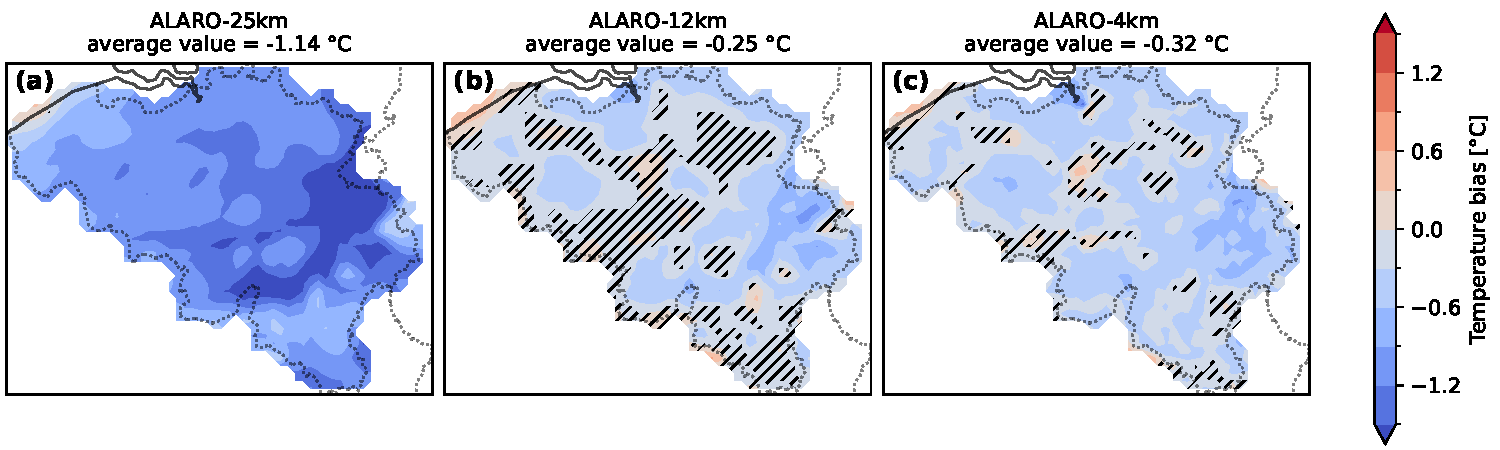
\includegraphics[width=\textwidth]{figures/fig02.pdf}
\caption{Bias in mean annual near-surface air temperature of each simulation (25 km, 12.5 km, and 4 km resolutions) with respect to the daily gridded observational CLIMATE-GRID dataset over Belgium.}
\label{fig:tas_bias}
\end{figure*}

Figure~\ref{fig:tas_bias} shows that ALARO-1 at all three resolutions exhibits a cold temperature bias with respect to the Belgian CLIMATE-GRID observations. 
This bias is most pronounced in the eastern, more elevated region. 
Near the coast, all simulations exhibit a small warm bias. 
The spatial bias patterns for ALARO-12km and ALARO-4km are very similar. 
Certain urban areas can be discerned in these simulations presenting themselves as areas with a warm bias. 

While the bias difference between ALARO-12km and ALARO-4km is small, a large difference is present between ALARO-25km and ALARO-12km. 
As outlined in Table \ref{tab:technical}, apart from the resolution difference, the primary distinction between these two simulations is the inclusion of SURFEX into ALARO-12km. 
These changes seem to considerably alter the current-day climatology, raising the temperature by nearly 1 $\degree$C.  Overall, ALARO-12km provides the best representation of mean annual temperature. 

Considering the annual cycle of the biases, a more complex picture emerges. 
The spatially averaged biases per month are plotted in Fig.~\ref{fig:bias_monthly}, while spatial bias patterns are shown per season in Fig.~\ref{fig:tas_bias_seasons}. 
In each season, ALARO-12km and ALARO-4km perform similarly, except during summer, when both simulations feature a warm bias which is larger in ALARO-12km, particularly in July and August when the bias exceeds 1°C. 
This warm bias partially compensates for the cold bias in other seasons on an annual basis. 
Consequently, ALARO-12km exhibits a smaller annual cold bias than ALARO-4km, despite ALARO-4km performing better in more seasons.
Additionally, both ALARO-12km and ALARO-4km strongly underestimate the temperature in spring, which also corresponds to the largest seasonal cold bias for ALARO-25km. 
The minimal bias, which is around -1.5°C, is attained in May. 
Finally, during the seasons with warming sea surface temperatures (SST), spring and summer, there is a cold bias near the coast, while the opposite is true for autumn and winter (see Fig.~\ref{fig:tas_bias_seasons}). 
This may be attributed to the monthly replacement of SST, creating a lag effect. 

%f
\begin{figure*}[t]
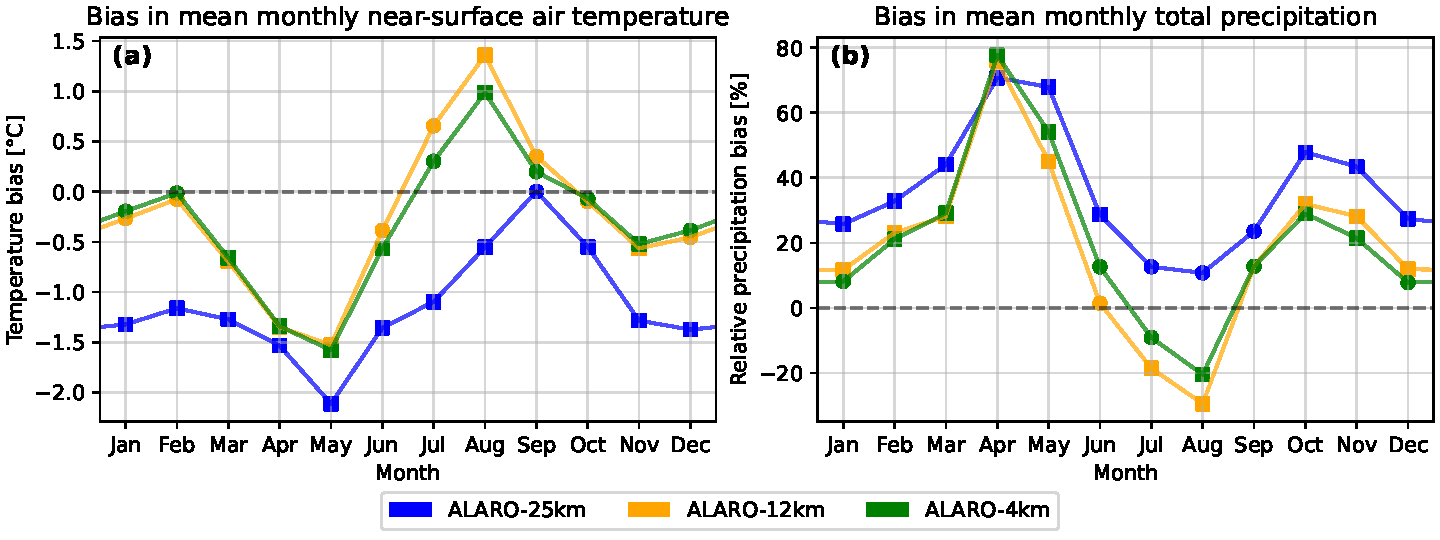
\includegraphics[width=\textwidth]{figures/fig03.pdf}
\caption{The annual cycle of the temperature bias (left) and relative precipitation bias (right) for each simulation (25 km, 12.5 km, and 4 km resolutions) with respect to the gridded observational CLIMATE-GRID dataset, averaged over Belgium.}
\label{fig:bias_monthly}
\end{figure*}

%f
\begin{figure*}[t]
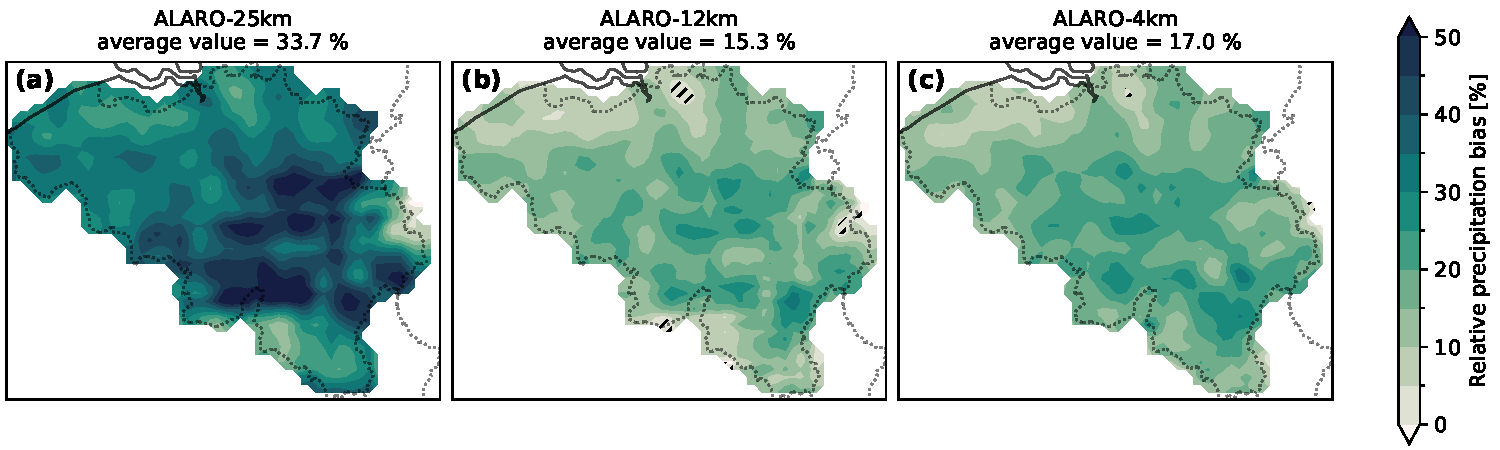
\includegraphics[width=\textwidth]{figures/fig04.pdf}
\caption{Relative bias in mean annual precipitation of each simulation (25 km, 12.5 km, and 4 km resolutions) with respect to the daily gridded observational CLIMATE-GRID dataset over Belgium.}
\label{fig:pr_bias}
\end{figure*}

ALARO-1, at all three resolutions, features a wet bias both annually (Fig.~\ref{fig:pr_bias}) and across all months (Fig.~\ref{fig:bias_monthly}) and seasons (Fig.~\ref{fig:pr_bias_seasons}). 
A notable exception is the dry bias in summer (July and August) in ALARO-12km and ALARO-4km, which coincides with a warm bias in these simulations. 
Similarly to temperature, the bias in annual precipitation is smallest for ALARO-12km. 
ALARO-4km is slightly wetter, while ALARO-25km features a bias nearly twice as high as ALARO-12km. 
However, once more, ALARO-4km performs best when evaluating the seasons separately. 
ALARO-12km shows a smaller bias only during springtime. 
Similarly to temperature, the precipitation bias in spring is substantially larger (in absolute values) compared to the other seasons. 

%f
\begin{figure*}[t]
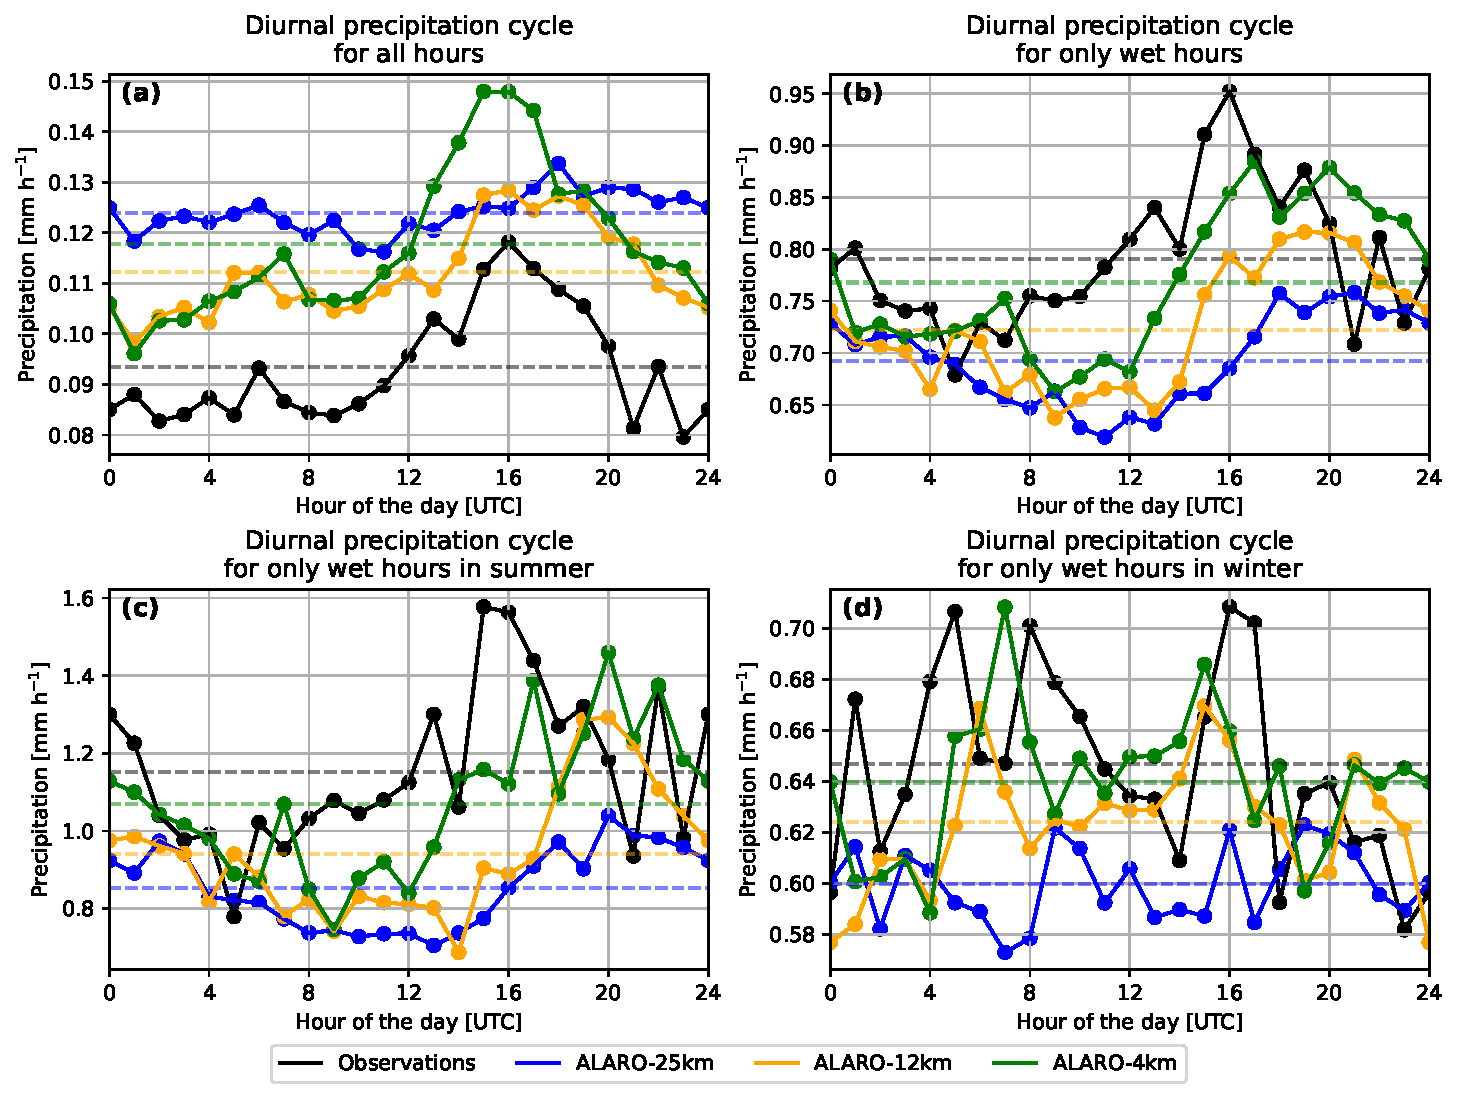
\includegraphics[width=\textwidth]{figures/fig05.pdf}
\caption{Diurnal cycle of precipitation in Uccle, Belgium, for station measurements (observations) and for each simulation (25 km, 12.5 km, and 4 km resolutions). The dashed lines denote the average values over the considered hours. (a) All hours. (b) Only wet hours (> 0.1 mm h$^{-1}$). (c) Only wet hours (> 0.1 mm h$^{-1}$), summer. (d) Only wet hours (> 0.1 mm h$^{-1}$), winter.}
\label{fig:pr_diurnal_cycle}
\end{figure*}

Figure~\ref{fig:pr_diurnal_cycle} shows the diurnal cycle of precipitation in Uccle, Belgium.
The diurnal cycle is first analyzed across all hours. 
All simulations overestimate rainfall for all hours. 
Apart from the systematic bias, ALARO-4km neatly reproduces the diurnal rainfall variation. 
The observed afternoon peak around 16 UTC, for instance, is also present in ALARO-4km albeit with a higher intensity.
ALARO-12km displays a smaller and slightly delayed peak, while ALARO-25km lacks a clear peak, maintaining roughly uniform precipitation amounts throughout the day. 
During wet hours (i.e. hours with a precipitation rate > 0.1 mm), on the other hand, there is a dry bias for all models.
ALARO-4km again aligns most closely with observations, followed by ALARO-12km and ALARO-25km. 
The afternoon peak at 16 UTC remains visible for the observations but is less pronounced and slightly delayed for ALARO-4km. 
The delay is even larger for ALARO-12km and ALARO-25km, with progressively smaller peaks as resolution decreases. 
In summer, average precipitation values and peak amplitudes are considerably higher, although the simulated peaks occur slightly later and are less intense at lower resolutions. 
In winter, no clear peak is observed, and the average precipitation intensity is approximately half of the summer values.
Overall, these results indicate that although the simulations reproduce the timing of the diurnal cycle reasonably well, they tend to overestimate precipitation frequency — raining too often with too little intensity — especially at coarser resolutions.

\subsection{Extreme precipitation}
\label{sect:extreme_precipitation}


%f
\begin{figure*}[t]
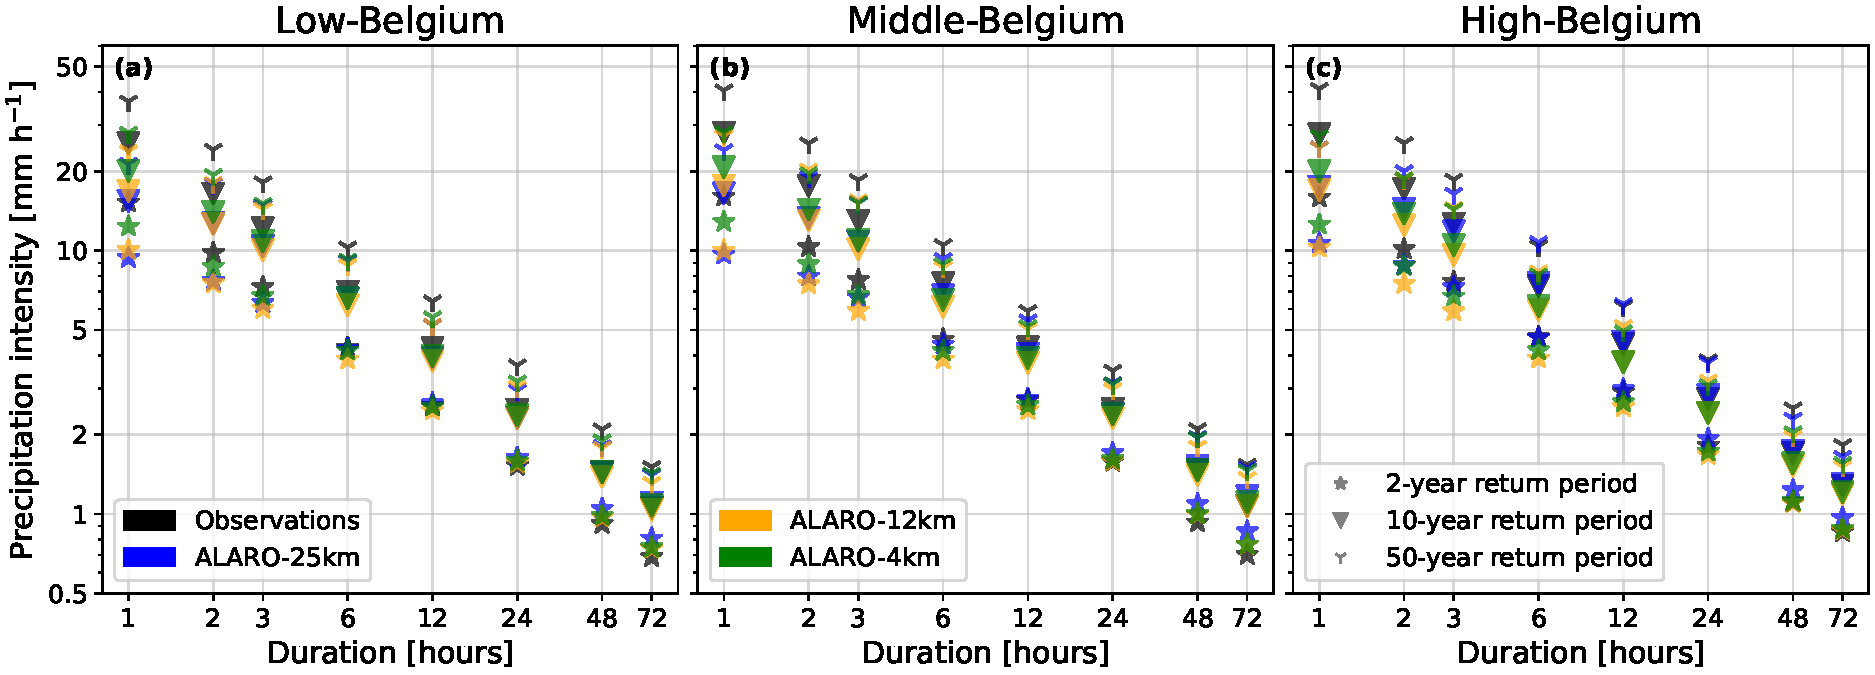
\includegraphics[width=\textwidth]{figures/fig06.pdf}
\caption{Intensity-Duration-Frequency (IDF) curves for three topographic regions over Belgium: Low-Belgium (<50m), Middle-Belgium (50m - 200m), and High-Belgium (>200m). The curves show the return level precipitation intensities for different durations, calculated using the Regional Frequency Analysis (RFA) framework. The colors represent the dataset: stations observations or simulations, while the markers represent the return levels for different return periods (2, 10, and 50 years).}
\label{fig:IDFs}
\end{figure*}

The calculated IDF-statistics are presented in Fig.~\ref{fig:IDFs} for each topographic region. 
The difference in observational return levels between the regions is apparent for both sub-daily durations (< 6h) and durations extending beyond one day (>= 24h). 
In the former case, the values for Middle- and High-Belgium are similar to one another, but those for Low-Belgium are smaller, while in the latter case, the difference between Middle- and Low-Belgium disappears and the return levels over High-Belgium exceed those over the other two regions. 

The observational return levels decrease linearly with rainfall duration on a log-log scale (see Fig.~\ref{fig:IDFs}).
For the simulated return levels, a linear relationship can also be discerned, except for short durations (< 6h), where the values start to curve downward, away from the observations. 
This effect is quantitatively assessed by evaluating the linear regression coefficients and $R^2$-values, as shown in Fig.~\ref{fig:IDFs_linear}.
The coefficients show that the observational return levels exhibit the steepest slope, followed by the simulations in order of decreasing resolution.
Furthermore, the fitted linear trend has a higher $R^2$-value for the observations, again followed by ALARO-4km, ALARO-12km and ALARO-25km, respectively.
Some differences can also be discerned for different return periods: overall, the return levels with a longer return period exhibit a steeper linear fit, but have a smaller $R^2$-value.

%f
\begin{figure*}[t]
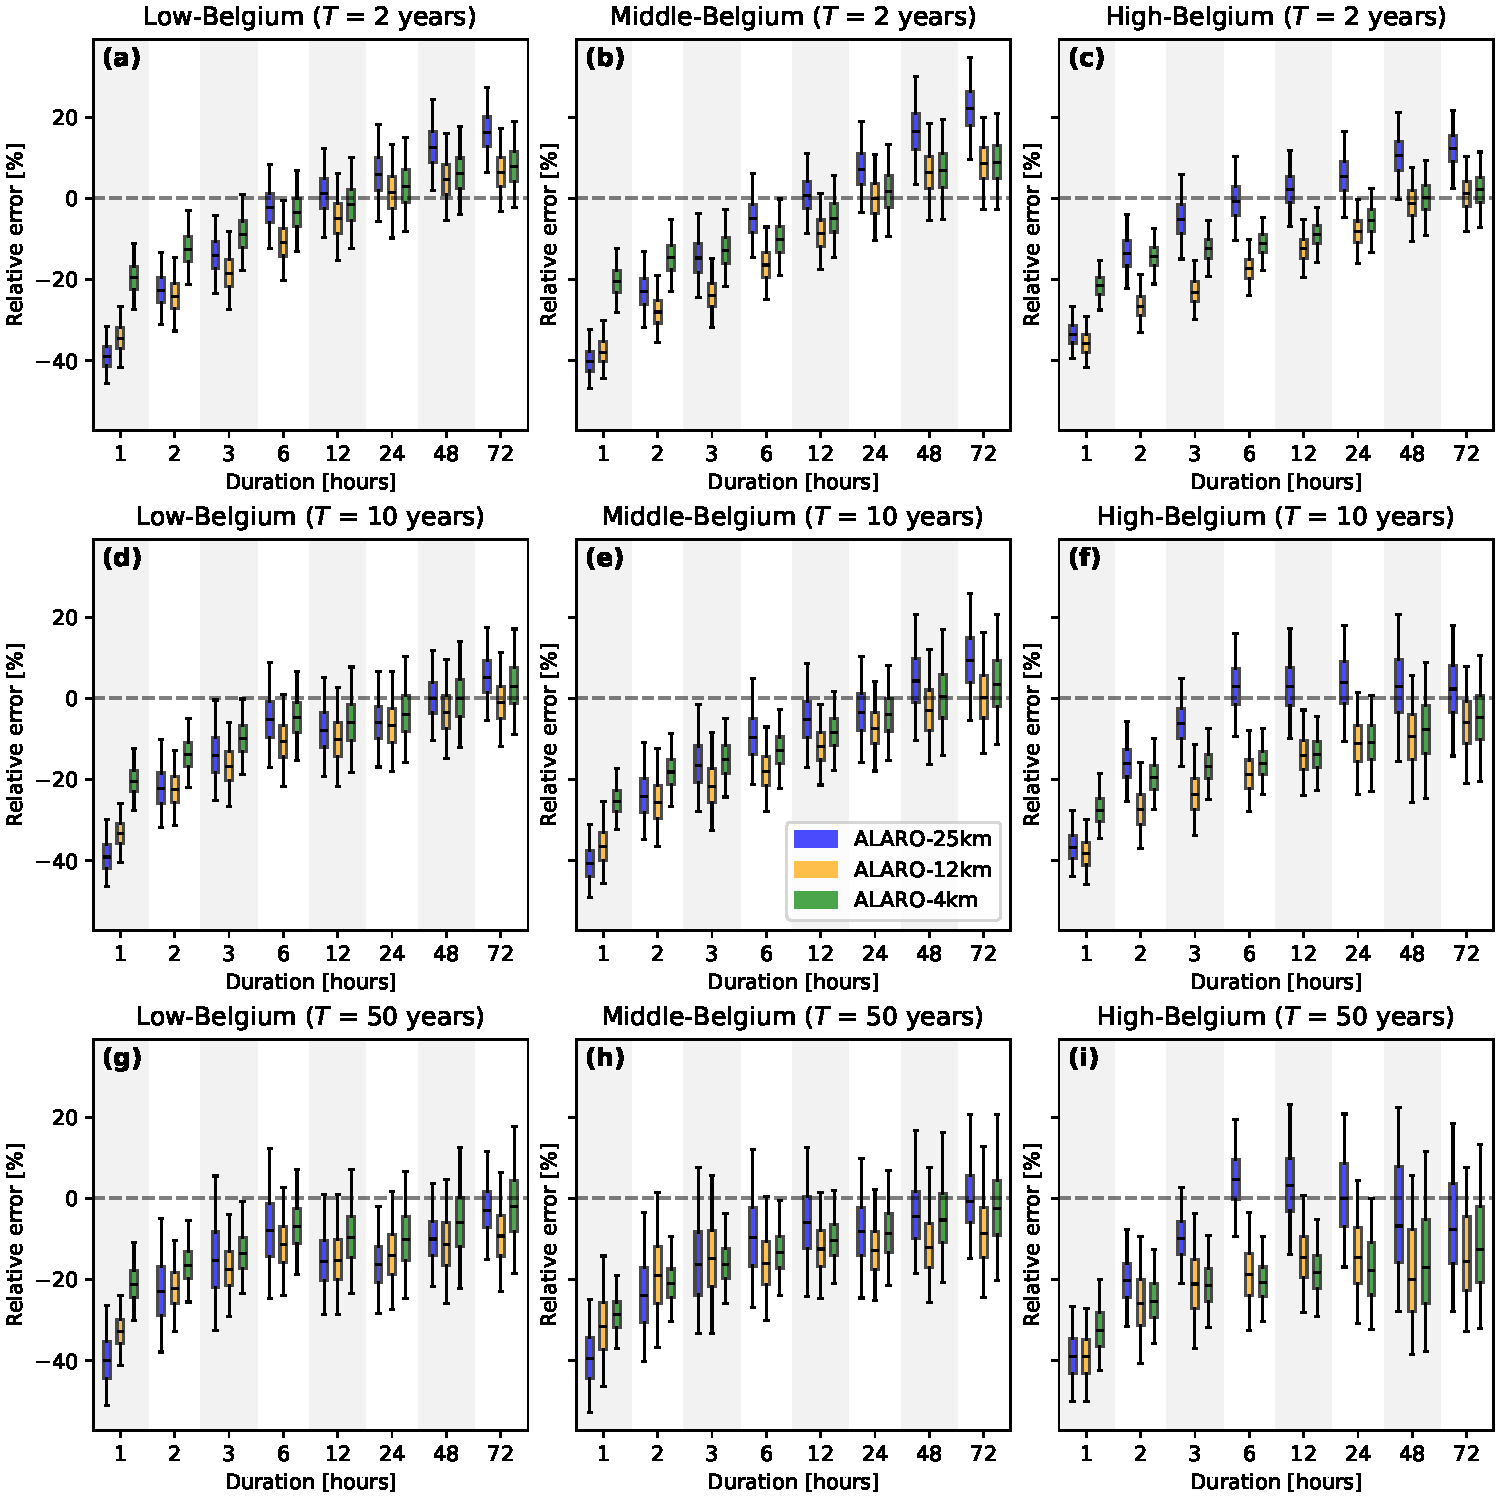
\includegraphics[width=\textwidth]{figures/fig07.pdf}
\caption{Relative error of the return-level intensities for each region (row) and return period (column). Each box plot represents the uncertainty as gauged by the bootstrap procedure with $10^4$ x $10^4$ ($= 10^8$) samples. The whiskers span the width of the 95 \%-confidence interval around the median.}
\label{fig:IDFs_boxplots}
\end{figure*}

Despite its strong wet bias for average rainfall, ALARO-25km underestimates the sub-daily (< 6h) return levels for all regions and return periods, as shown in Fig.~\ref{fig:IDFs_boxplots}. 
For the  (multi-)daily (>= 24h) durations, the performance depends on the return period. 
The least extreme events i.e. those with the shortest return period, are overestimated, while the events with the longest return period generally tend to be underestimated, although the uncertainty was large. 
Conversely, ALARO-12km provides smaller return levels than ALARO-25km for sub-daily (< 6h) durations, except for hourly events in Low- and Middle-Belgium. 
Hence, the sub-daily extreme precipitation intensities are also underestimated by this simulation. 
For (multi-)daily (>= 24h) durations, this intensity decrease with higher resolution is also present, especially in High-Belgium. 
Finally, for ALARO-4km the hourly return levels are substantially closer to the observational values for a 2-year return period and markedly closer for longer return periods.
Generally, the ALARO-4km extremes increase compared to the ALARO-12km simulation, leading to improvements for some durations and regions, but not universally.

%f
\begin{figure*}[t]
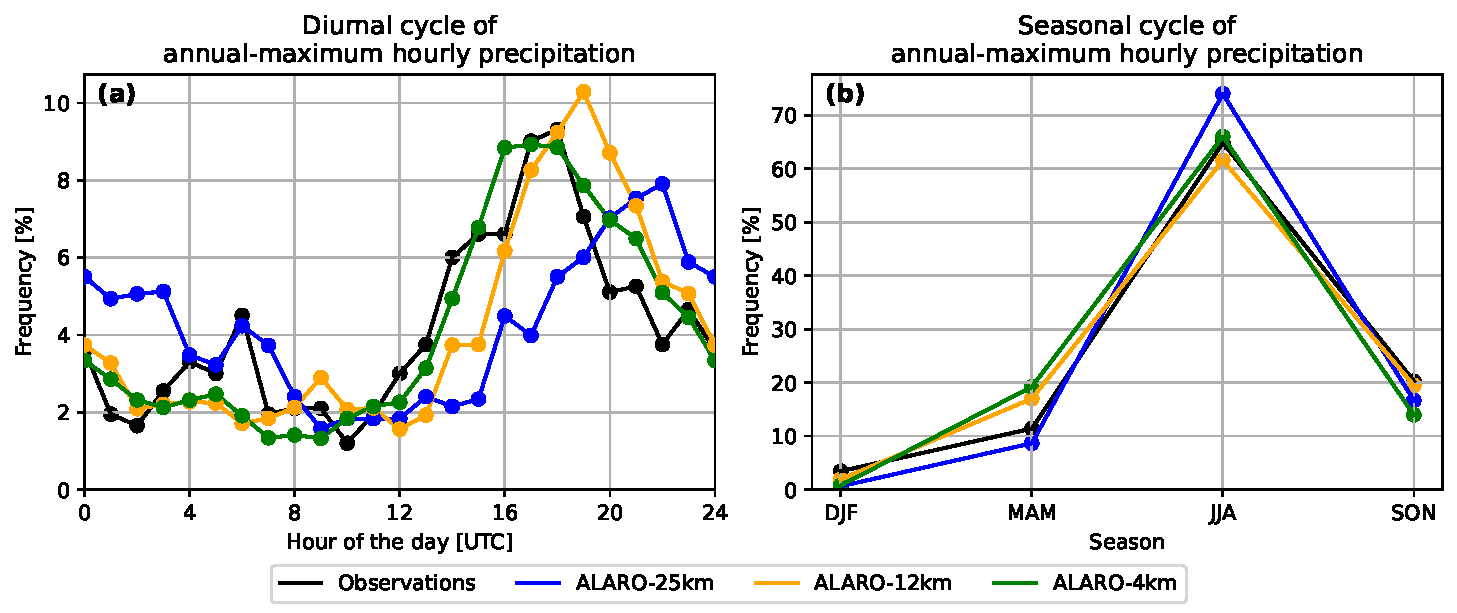
\includegraphics[width=\textwidth]{figures/fig08.pdf}
\caption{Frequency of annual-maximum hourly precipitation intensities over Belgium for hourly station observations (HYDRO network) and for each simulation (25 km, 12.5 km, and 4 km resolutions). (left) Diurnal cycle: showing the frequency of annual-maximum hourly precipitation intensities for each hour of the day (UTC). (right) Seasonal cycle: showing the frequency of annual-maximum hourly precipitation intensities for each season (winter, spring, summer, autumn).}
\label{fig:AMcycles}
\end{figure*}

Figure~\ref{fig:AMcycles} presents the diurnal and seasonal cycles of the frequency of annual-maximum hourly precipitation intensities over Belgium. 
In the diurnal cycle, the observations clearly show a primary peak in the afternoon. 
ALARO-4km captures both the timing and magnitude of this peak with high accuracy. 
ALARO-12km also reproduces a peak, but it occurs slightly later (i.e. 1-2 hours) and with a higher frequency than observed. 
For ALARO-25km, the peak occurs even later (around 22:00 UTC) and has a lower frequency compared to the observations.
Furthermore, the observational data reveal a secondary peak in the early morning, which is absent in all simulations.
Although ALARO-25km appears to align with the observed morning peak, this is primarily due to elevated nighttime frequencies in the simulation rather than a distinct early morning peak.

\section{Discussion}
\label{sect:discussion}

\subsection{Validation of average climatology}

A clear distinction in climatology can be drawn between ALARO-25km on the one hand, and ALARO-12km and ALARO-4km on the other hand, both for near-surface air temperature and accumulated precipitation. 
The cold bias from ALARO-25km of -1.14 $\degree$C over Belgium is significantly improved by about 1 $\degree$C in the two simulations with the highest resolutions, as shown in Fig.~\ref{fig:tas_bias}. 
Furthermore, these simulations both exhibit a reduced wet bias in comparison with ALARO-25km. 
The difference between ALARO-12km and ALARO-4km is mostly small when compared to ALARO-25km.
Aside from the difference in resolution, ALARO-12km employs the land-surface model SURFEX, while ALARO-25km still uses the built-in module ISBA. 
This difference in configuration might explain the clear distinction between these two sets of simulations.

In~\citet{giot_validation_2016} 30-year simulations over Europe were performed with ALARO-0, a previous version of the ALARO model, and the built-in land surface scheme ISBA.
These simulations were performed at resolutions of 0.44$\degree$ ($\sim 50$ km) and 0.11$\degree$  ($\sim 12$ km) and contained an area-averaged yearly bias in near-surface air temperature of a little less than -1°C over the Middle-European sub-region (which covers Belgium, the Netherlands, most of Germany, and parts of neighbouring countries).
This result is very similar to the yearly bias of ALARO-25km in this work.
The seasonal temperature biases of~\citet{giot_validation_2016} over Middle-Europe are also in line with the results of ALARO-25km. 

Furthermore, in~\citet{berckmans_reinitialised_2017}, simulations with ALARO-0 for a 10-year period were carried out in three different configurations, one of which consisted of continuous simulations as performed in this work. 
It should be noted that, contrary to those of~\citet{giot_validation_2016}, these simulations were performed with the SURFEX model, albeit a previous version, SURFEXv5. 
Over Middle-Europe, an average yearly temperature bias of -1.6 °C was found, while for winter and summer a bias of -1.3 °C was presented.
This is comparable to the results of~\citet{giot_validation_2016} and of ALARO-25km, even though the latter simulations did not use SURFEX.

Lastly, 4 km ALARO-0 simulations without SURFEX were performed in the context of the CORDEX.be I project~\citep{termonia_cordexbe_2018}. 
In the final report~\citep{termonia_combining_2018} a cold bias of 1.3 °C in the average yearly temperature over Belgium was presented. 
This value is in line with the results from~\citet{giot_validation_2016},~\citet{berckmans_reinitialised_2017}, and ALARO-25km, 
but contrasts with the temperature bias of the here-presented ALARO-12km and ALARO-4km, even though these CORDEX.be I simulations were run at 4 km. 
This suggests that the use of SURFEX is responsible for the improved temperature bias.

Evaluation against the CG dataset reveals that all ALARO-1 simulations exhibit a consistent annual wet bias over Belgium, with this bias most pronounced in ALARO-25km. 
Seasonal analyses confirm a wet bias across all seasons, except for a dry bias in summer in both ALARO-12km and ALARO-4km. 
Differences between ALARO-12km and ALARO-4km remain insubstantial across seasons.
These patterns indicate that the inclusion of SURFEX exerts a greater influence on average precipitation than changes in spatial resolution.

Our results for rainfall (Fig.~\ref{fig:pr_bias}) are now compared to previous continuous simulations from~\citet{giot_validation_2016} (resolutions of 50 and 12.5 km).
The annual bias from ALARO-25km is slightly larger than the bias over Middle-Europe (ME) from~\citet{giot_validation_2016}, while for ALARO-12km and ALARO-4km it is smaller.
On the other hand, the annual precipitation bias over ME in~\citet{berckmans_reinitialised_2017} (at 20 km resolution) was 15$\%$, which agrees almost perfectly with the results from ALARO-12km and ALARO-4km. 
For summer and winter precipitation, the biases of~\citet{berckmans_reinitialised_2017} and~\citet{giot_validation_2016} are similar to each other and resemble closely those of ALARO-25km. 
Conversely, the winter, and particularly the summer precipitation totals are much drier in ALARO-12km and ALARO-4km compared to ALARO-25km.
The large wet bias in spring, reported in~\citet{giot_validation_2016} is also present (and slightly increased) in the simulations in this work.
Finally, the large bias in autumn was absent in the simulations of~\citet{giot_validation_2016}, where the bias was between 0 and 10$\%$.

Previous 4 km simulations showed results similar to ALARO-4km.
Compared to the HRES-simulations from CORDEX.be I, the bias in winter precipitation was of comparable magnitude~\citep{termonia_combining_2018}.
Biases from~\citet{de_troch_multiscale_2013} were slightly smaller for summer precipitation than for ALARO-4km: their 4 km simulation showed a bias of only 3\%.
Notably, those simulations employed daily restarts, which could have a significant impact—especially in summer, when soil moisture feedbacks tend to play a more important role.
There was a difference of roughly 10 percentage points between their 10 km and 4 km simulations in summer precipitation bias, which is also present between ALARO-12km and ALARO-4km but with an opposite sign. 
Both cases can be interpreted as an improvement in the representation of (convective) precipitation when increasing the resolution. 

In~\citet{de_troch_application_2016}, the multi-scale behaviour of ALARO-0 was investigated by means of the diurnal cycle of precipitation in summer and winter.
An identical distinction between all hours and wet hours is made in this work, as shown in Fig.~\ref{fig:pr_diurnal_cycle}. 
It was shown in~\citet{de_troch_application_2016} that in summer the timing and amplitude of the diurnal peak were improved for simulations with ALARO-0 at 10 and 4 km compared to a 40 km simulation, when considering all hours. 
However, the timing of the afternoon peak as reproduced by the model was still too early. 
A similar behaviour is evident in this work, although ALARO-4km captures the timing better (later) than in~\citet{de_troch_application_2016}.
For winter precipitation, the 4 km simulation from~\citet{de_troch_application_2016} exhibited a weak peak in the early afternoon, which is absent in the observations. 
Our ALARO-4m simulations reproduce this constant diurnal pattern better than those in \citet{de_troch_application_2016}.

When considering only wet hours (i.e. hours with a precipitation rate > 0.1 mm), the observations show no diurnal variation (regardless of some noise) in winter. 
All simulations in this paper reproduce this pattern, with the mean precipitation increasing towards the observed value as the resolution increases.
For wet hours in summer, all simulations contain an afternoon/evening peak, with increasing amplitude for higher resolutions, similar to the study of~\citet{de_troch_application_2016}. 
The timing of the peak does not significantly differ between ALARO-25km and ALARO-12km, and is slightly earlier for ALARO-4km. 
However, for all simulations, the diurnal peak is later than the observational peak, which is in contrast with results from~\citet{de_troch_application_2016}. 
Overall, for both all-hour and wet-hour precipitation, the diurnal cycles in ALARO-4km are comparable to those in the work of~\citet{de_troch_application_2016}.

In our analysis of the mean diurnal precipitation cycle, notable differences emerge when comparing simulations at varying resolutions with observational data, as shown in Fig.~\ref{fig:pr_diurnal_cycle}. 
Specifically, while the ``all-hour'' precipitation cycle tends to exhibit an overestimation relative to observations, the ``wet-hour'' cycle shows a general underestimation.
This implies that the precipitation frequency is overestimated. 
This discrepancy is most pronounced in the ALARO-25km simulation and is minimized in the ALARO-4km simulation, indicating that the coarser resolution more significantly overestimates precipitation amounts due to an overly high rainfall frequency. 
These results imply that drizzle contributes substantially to the simulated rainfall, particularly in the lower-resolution model.
This problem is partially mitigated when using CPMs, but not entirely.
ALARO-4km still exhibits a drizzle bias, even at scales where convection is (partially) permitted by the scale-aware convection scheme 3MT.
This finding is consistent with previous works~\citep{kendon_realism_2012, fosser_benefit_2015, berthou_pan-european_2020}.
Additionally, it has been shown that both the timing and amplitude of the diurnal precipitation peak are best represented at high resolution. 
This result is well established for CPMs, as documented by numerous studies referenced in the review of~\citet{lucas-picher_convection-permitting_2021}. 
Most RCMs tend to exhibit a premature diurnal peak, primarily due to the limited memory of atmospheric instabilities. 
However, this behaviour is notably absent in this study. 
At lower resolutions, the diurnal peak in ALARO even occurs later than at higher resolutions. 
This difference may be attributable to the scale-aware character of the 3MT scheme. 

\subsection{Extreme precipitation}

IDF curves are presented in Fig.~\ref{fig:IDFs} for durations of 1 to 72 hours across three distinct topographic regions in Belgium.
The regional differences in return levels, with smaller sub-daily (< 6h) values in Low-Belgium and higher (multi-)daily (>= 24h) values in High-Belgium, are consistent with the findings of~\citet{van_de_vyver_practical_2013}.
In each case, the return levels scale linearly with duration on a log-log scale, for both observations and simulations.
This corresponds to a power-law relationship on a linear scale and reflects the underlying scale invariance and multifractal characteristics of extreme precipitation.
These phenomena can be effectively captured using simple scaling techniques, which in turn result in a power-law relationship~\citep{gupta_multiscaling_1990, veneziano_multifractality_2002}.
However, for short rainfall durations (1--3 hours), simulated return levels deviate from this linear trend, curving downward, whereas observational return levels do not exhibit this pattern.
This discrepancy arises entirely from model error, as precipitation values from both observations and simulations were first aggregated to an hourly resolution before extracting the annual maxima.
As shown in Fig.~\ref{fig:IDFs_linear}, the smaller $R^2$-values indicate a less optimal fit for larger spatial scales.
The higher (less negative) linear coefficients at these scales may also reflect this underestimation at short durations.
However, previous studies have also shown that annual-maximum precipitation at larger spatial scales has a higher linear coefficient with respect to duration than at smaller scales~\citep{innocenti_observed_2019}.
Next, these linear coefficients can be compared to those from a simple-scaling model by~\citet{van_de_vyver_multiscalingbased_2018}.
In that work, station-specific values in the range of $-0.75$ and $-0.64$ were found for 16 stations over Belgium.
The observational coefficients depicted in Fig.~\ref{fig:IDFs_linear} correspond to this range, although they are slightly more negative.

At durations of 1 to 3 hours, lower-resolution simulations increasingly underestimate return levels compared to observational values, highlighting the added value of the convection-permitting ALARO-4km simulation. 
A similar result was found by~\citet{tabari_local_2016}, who also constructed IDF curves for ALARO-0 simulations at different resolutions. 
In that study, the 4 km and 10 km ALARO-0 simulations accurately captured sub-daily intensities, with a slight underestimation, while ALARO-40km significantly underestimated sub-daily precipitation amounts. 
For longer durations (>24 hours), ALARO-25km tends to overestimate return levels, particularly for short return periods. 
\citet{de_troch_application_2016} reported a similar finding, as all ALARO-0 simulations (4 km, 10 km, and 40 km) overestimated the 2-year return level for daily precipitation. 
Additionally, while~\citet{de_troch_application_2016} observed increasing overestimation for longer return periods in the 4 km ALARO-0 simulation, this effect is notably absent - and even reversed - in ALARO-4km.

Because of the scale-aware design of the 3MT scheme, the statistics of extreme precipitation should, in principle, be independent of model resolution. 
In previous studies~\citep{de_troch_application_2016, tabari_local_2016}, return levels exhibited a gradual change with resolution, which is broadly consistent with the expected resolution independence. 
In contrast, the return levels presented in this study display a more abrupt, step-wise change when transitioning from 12 km to 4 km resolution. 
This behaviour is more similar to that observed in other models without a scale-aware convective scheme, where the step-wise shift is typically attributed to the deactivation of the deep convective parameterization at high resolutions.

The diurnal cycle of hourly AM precipitation frequencies is well captured by ALARO-4km (see Fig.~\ref{fig:AMcycles}).
Both the frequency peak amplitude and timing are in agreement between ALARO-4km and the observational data.
The peak occurs later in ALARO-12km and is further delayed in ALARO-25km, while the peak amplitude increases in ALARO-12km but decreases in ALARO-25km.
This peak delay is also present in $0.11\degree$ EURO-CORDEX simulations~\citep{meredith_present_2021}.
It should be noted that the relatively large diurnal variation in extreme rainfall frequency of ALARO-25km is quite remarkable, as most models exhibit almost no diurnal variation at similar resolutions~\citep{meredith_present_2021, thomassen_spatial_2023}.
The diurnal cycle of extremes from previous ALARO-0 simulations at 12 km and 4 km was shown in~\citet{van_de_vyver_evaluation_2021}. 
However, they did not find a large difference in the diurnal cycle between both resolutions, in contrast to the simulations of this work. 

Similarly to the diurnal cycle, the seasonal cycle of hourly extreme-precipitation frequency is well captured by our three simulations, as shown in Fig.~\ref{fig:AMcycles}.
The frequency peak in summer due to the convective nature of hourly extreme precipitation is apparent.
This result corresponds to previous simulations from~\citet{van_de_vyver_evaluation_2021}, who also did not find a difference in the seasonal cycle between 12 km and 4 km ALARO-0 simulations.
In contrast,~\citet{innocenti_observed_2019} reported the slight outperformance of a 12 km RCM simulation compared to a 4 km convection-permitting WRF simulation in capturing the seasonal cycle of hourly AM occurrences over North America.

\conclusions  %% \conclusions[modified heading if necessary]
\label{sect:conclusions}

%% The following commands are for the statements about the availability of data sets and/or software code corresponding to the manuscript.
%% It is strongly recommended to make use of these sections in case data sets and/or software code have been part of your research the article is based on.

This study evaluated the performance of the ALARO-1 model, including a scale-aware deep convection parameterization, over Belgium using a multi-level dynamical downscaling framework at three horizontal resolutions: 25 km, 12.5 km, and 4 km.
The ALARO-1 model was coupled online to the land-surface model SURFEX v8.0 for ALARO-12km and ALARO-4km.
These simulations, spanning a 32-year period (1991–2022), were compared against both a gridded observational dataset (CLIMATE-GRID) and hourly precipitation values from station measurements.

The analysis of average climatology demonstrated that across all resolutions the ALARO-1 model exhibits an annual cold bias between -1.14 $\degree$C and -0.25 $\degree$C and an annual wet bias between 15.3 \% and 33.7 \% over Belgium.
Comparing resolutions, ALARO-12km and ALARO-4km outperformed ALARO-25km, which exhibited larger biases in both temperature and precipitation.
While ALARO-12km and ALARO-4km provided similar results in terms of average climatology, ALARO-4km captured the diurnal cycle of precipitation better.

A key focus of this study was the representation of extreme precipitation, evaluated through Intensity-Duration-Frequency curves derived from annual maximum precipitation.
While all simulations followed the expected log-log linear behaviour between return-level precipitation intensity and duration, lower-resolution models underestimated return levels at sub-daily timescales.
ALARO-4km significantly improved upon this, producing more realistic hourly return levels and better capturing the diurnal timing of hourly extreme precipitation.
These findings provide clear experimental evidence that increasing model resolution enhances the simulation of extreme precipitation.

Despite these improvements, this study has some limitations. 
The research domain was limited to Belgium due to computational constraints.
Another limitation is the absence of simulations at even higher resolutions, which could further improve model accuracy but are currently also constrained by computational demands.

Future research should address these challenges by conducting simulations at resolutions higher than 4 km and applying the ALARO-1 model to regional downscaling of global climate models (GCMs) and climate projections.
Additionally, a more detailed investigation of the urban effect on temperature and precipitation, as represented by the TEB model in SURFEX, is warranted.
Expanding the application of the ALARO-1 model to other regions would further validate its performance.
Finally, given the high computational cost of convection-permitting simulations, future work should explore alternative, more targeted downscaling approaches to reduce computational demands while maintaining or improving model accuracy, specifically for extreme precipitation.

\appendix

\section{Definition of bias}
\label{sect:bias_definition}

The temperature and precipitation bias are calculated in the following way. Let $X_{kni}$ be the value of variable $X$ at time $k$, with $k = 1, \ldots, K$, in grid point $n$, with $n = 1, \ldots, N$, and in year $i$, with $i = 1$. We define the total value of $X$ over a period $t$ as:
\begin{equation*}
    X^t_{ni} = \sum_{k \in t} X_{kni}
\end{equation*}
The average value over a period $t$ is defined as:
\begin{equation*}
    \bar{X}^t_{ni} = \frac{1}{K_t} \sum_{k \in t} X_{kni}
\end{equation*}
with $K_t$ the number of values in period $t$: $K_t = \sum_{k \in t} 1$

In this work, we consider three types of periods $t$: (1) months, denoted as $m \in M$ with $M = \{\text{Jan}, \text{Feb}, \text{Mar}, \text{Apr}, \text{May}, \text{Jun}, \text{Jul}, \text{Aug}, \text{Sep}, \text{Oct}, \text{Nov}, \text{Dec} \}$ (2) seasons, denoted as $s \in S$ with $S = \{\text{DJF}, \text{MAM}, \text{JJA}, \text{SON} \}$, and (3) years, denoted as $y$. The yearly total value of $X$ is related to the seasonal values as:
\begin{equation*}
    X^y_{ni} = \sum_{s} X^s_{ni}
\end{equation*}
and the yearly averaged value:
\begin{equation*}
    \bar{X}^y_{ni} = \frac{1}{4} \sum_{s} \bar{X}^s_{ni}
\end{equation*}

Let $\bar{T}^{t}_{ni}$ now be the temperature averaged over the period $t$, with $t \in (M \cup S \cup \{y\})$. The temperature bias is consequently calculated by taking the difference between the model temperature $T^{t,m}_{ni}$ and the observational temperature $T^{t,o}_{ni}$ with $t \in (M \cup S \cup \{y\})$ and averaging it over all years $i$ (with $I$ the number of years). The bias in grid point $n$ is hence:
\begin{equation*}
    \bar{T}^{x,b}_{n} = \frac{1}{I} \sum_{i} \left(\bar{T}^{x,m}_{ni} - \bar{T}^{x,o}_{ni} \right)
\end{equation*}
The spatially averaged bias is then acquired by averaging over all grid points (with $N$ the number of grid points):
\begin{equation*}
    \bar{T}^{t,b} = \frac{1}{N} \sum_{n} \bar{T}^{t,b}_{n} 
\end{equation*}
The seasonal and annual values can be straightforwardly related to each other:
\begin{equation*}
    \bar{T}^{y,b} = \frac{1}{4} \sum_{s} \bar{T}^{s,b}
\end{equation*}

For precipitation, we consider the relative bias. Let $P^{t}_{ni}$ now be the total precipitation over the period $t$ with $t \in (M \cup S \cup \{y\})$. The relative bias over this period is then calculated as:
\begin{equation*}
    P^{t,r}_{n} = \frac{ \sum_{i} \left(P^{t,m}_{ni} - P^{t,o}_{ni} \right)}{\sum_{i} P^{t,o}_{ni}}
\end{equation*}
The spatially averaged value then becomes:
\begin{equation*}
    P^{t,r} = \frac{1}{N} \sum_{n} P^{t,r}_{n}
\end{equation*}
For the relative bias, there is no straightforward relation between annual and seasonal values: 
\begin{equation*}
    P^{y,r} \neq \sum_{s} P^{s,r}
\end{equation*}

\section{Definition of GEV distribution}
\label{sect:gev_definition}

The cumulative GEV distribution function (for $\xi \neq 0$) is given by: 
\begin{equation}
    F(x) = \exp \left\{- \left[1 + \xi \left(\frac{x - \mu}{\sigma} \right) \right]^{-1/\xi} \right\}
\label{eq:GEV}
\end{equation}
The distribution with $\xi = 0$ is then interpreted as the limit of Eq. (\ref{eq:GEV}) as $\xi \to 0$:
\begin{equation}
    F(x) = \exp \left\{- \exp \left[- \left(\frac{x - \mu}{\sigma} \right) \right] \right\}
\label{eq:GEV0}
\end{equation}

GEV distribution functions are constructed for each duration separately. We denote the duration-specific GEV parameters as $\xi_d$, $\mu_d$, and $\sigma_d$. Subsequently, these distribution functions are used to calculate return levels $z_d(T)$ for the precipitation intensity. A return level $z_d(T)$ (expressed in mm h$^{-1}$) is specified for a certain return period $T$ and duration $d$. It is defined as the precipitation intensity which has a probability of $1/T$ of being exceeded in any given year: so on average once every $T$ years. The formula for these return levels can be derived from equations (\ref{eq:GEV}) and (\ref{eq:GEV0}):
\begin{equation}
    z_d(T) = \mu_d - \frac{\sigma_d}{\xi_d} \left\{1 - \left[- \ln{\left(1 - \frac{1}{T} \right)} \right]^{-\xi_d} \right\}
\end{equation}

\newpage

\section{Station data specifications}

\begin{table*}[h!]
\caption{Specifications of observational networks used in this study.}
\begin{tabular}{lcc}
\tophline
Network name & Number of years (start year - end year) & Number of locations \\
\middlehline
DGH & 20 (2004 -- 2003) & 95 \\
VMM & 11 (2013 -- 2023) & 36 \\
AWS & 24 (2000 -- 2023) & 13 \\
HYDRO & 38 (1967 -- 2004) & 18 \\
IBGE & 19 (1992 -- 2010) & 14 \\
\bottomhline
\end{tabular}
\belowtable{} \label{tab:stations}
\end{table*}

\newpage

\section{Additional figures}    
\subsection{Validation of average climatology}
\begin{figure*}[h!]
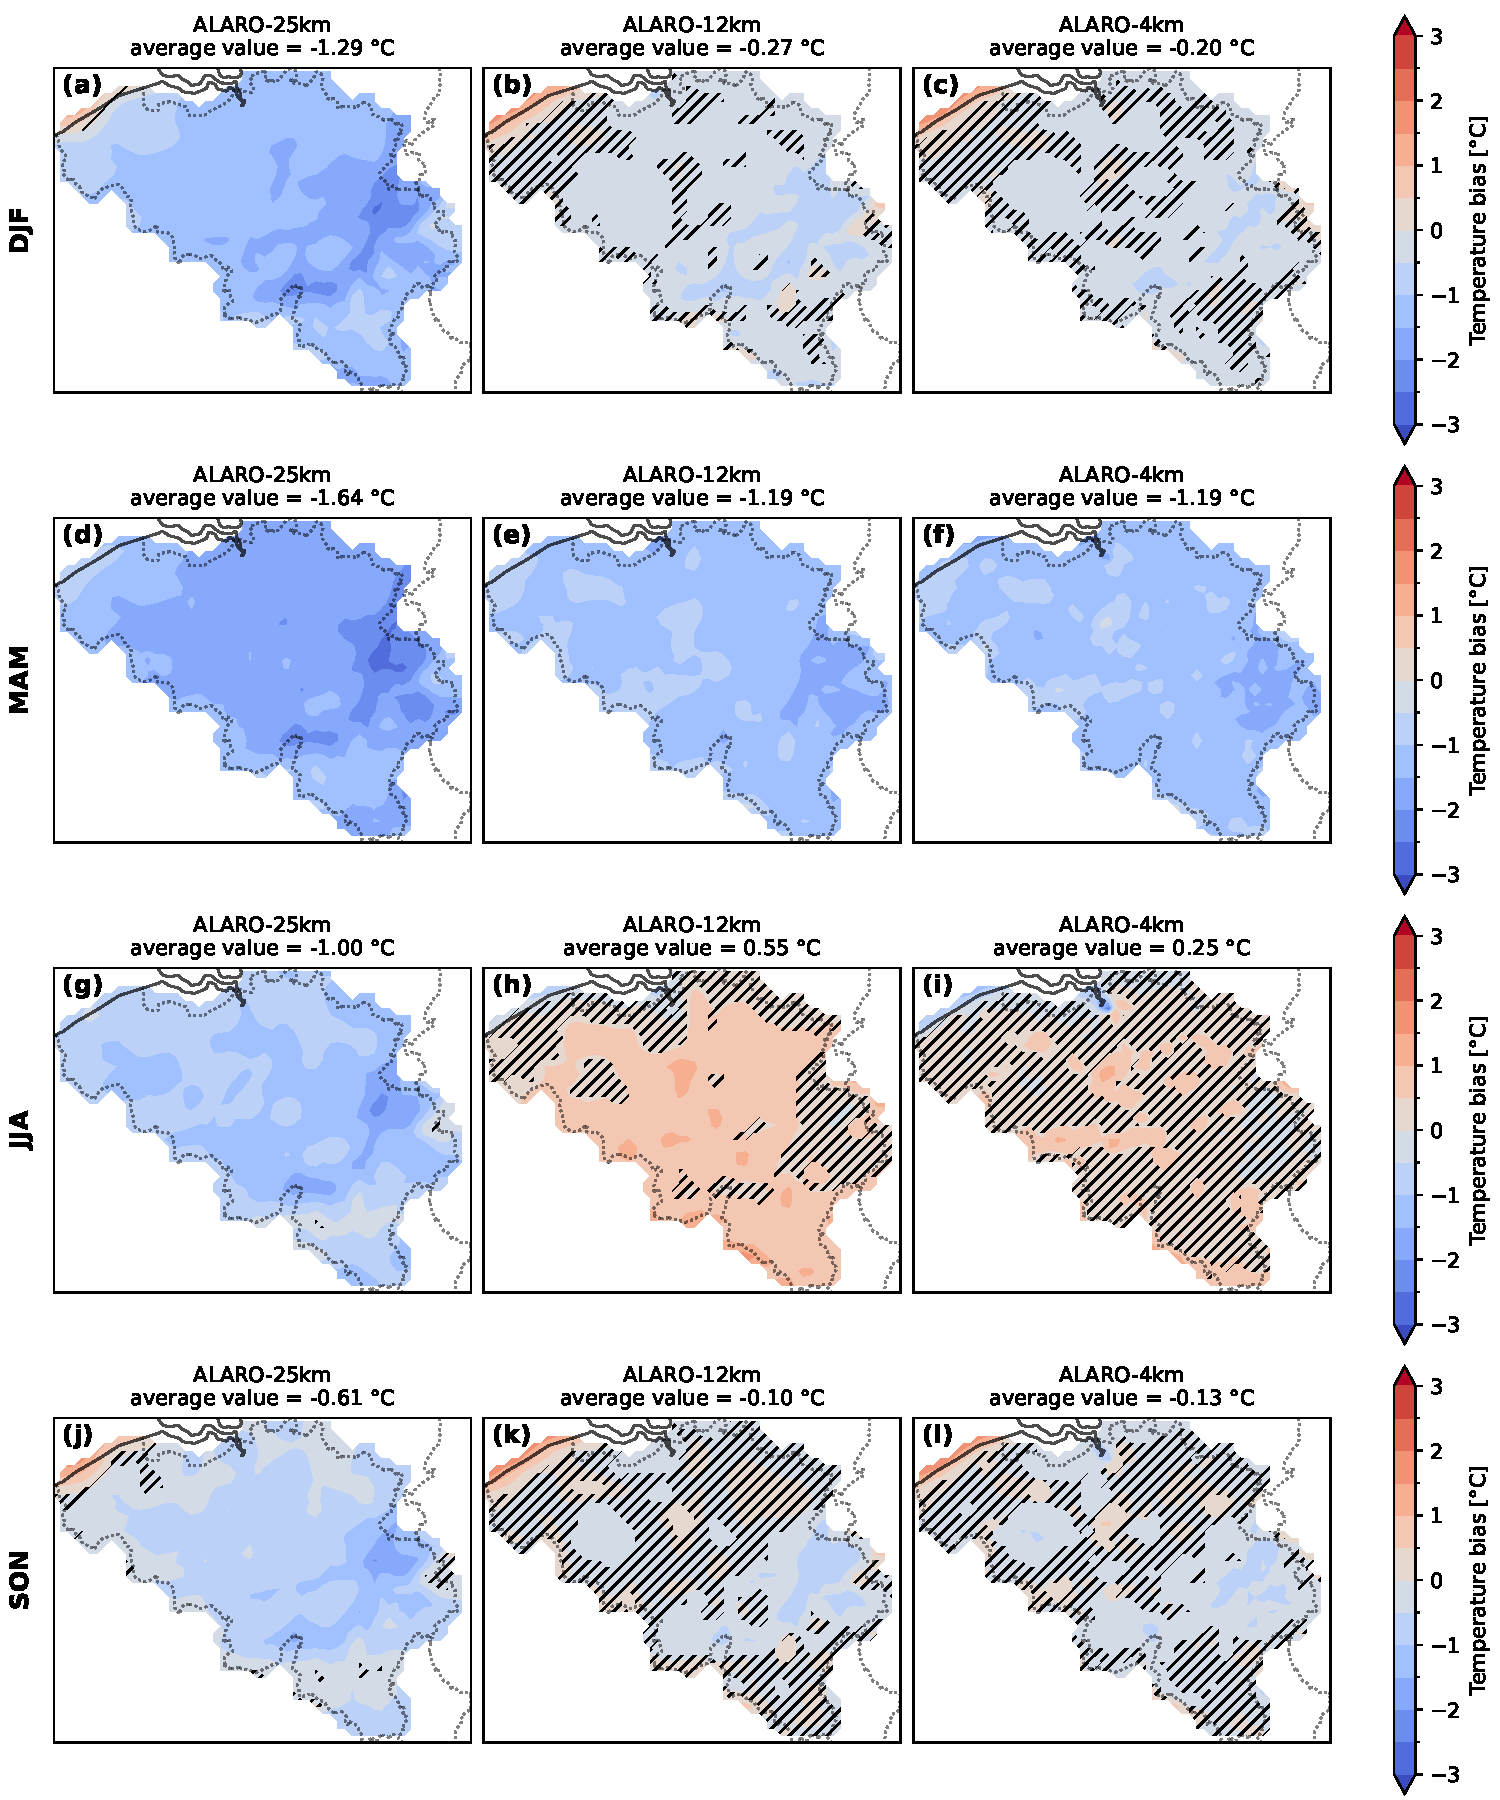
\includegraphics[width=12cm]{figures/figD1.pdf}
\caption{Bias in mean seasonal near-surface air temperature of each simulation (25 km, 12.5 km, and 4 km resolutions) with respect to the daily gridded observational CLIMATE-GRID dataset over Belgium.}
\label{fig:tas_bias_seasons}
\end{figure*}
\newpage
\begin{figure*}[h!]
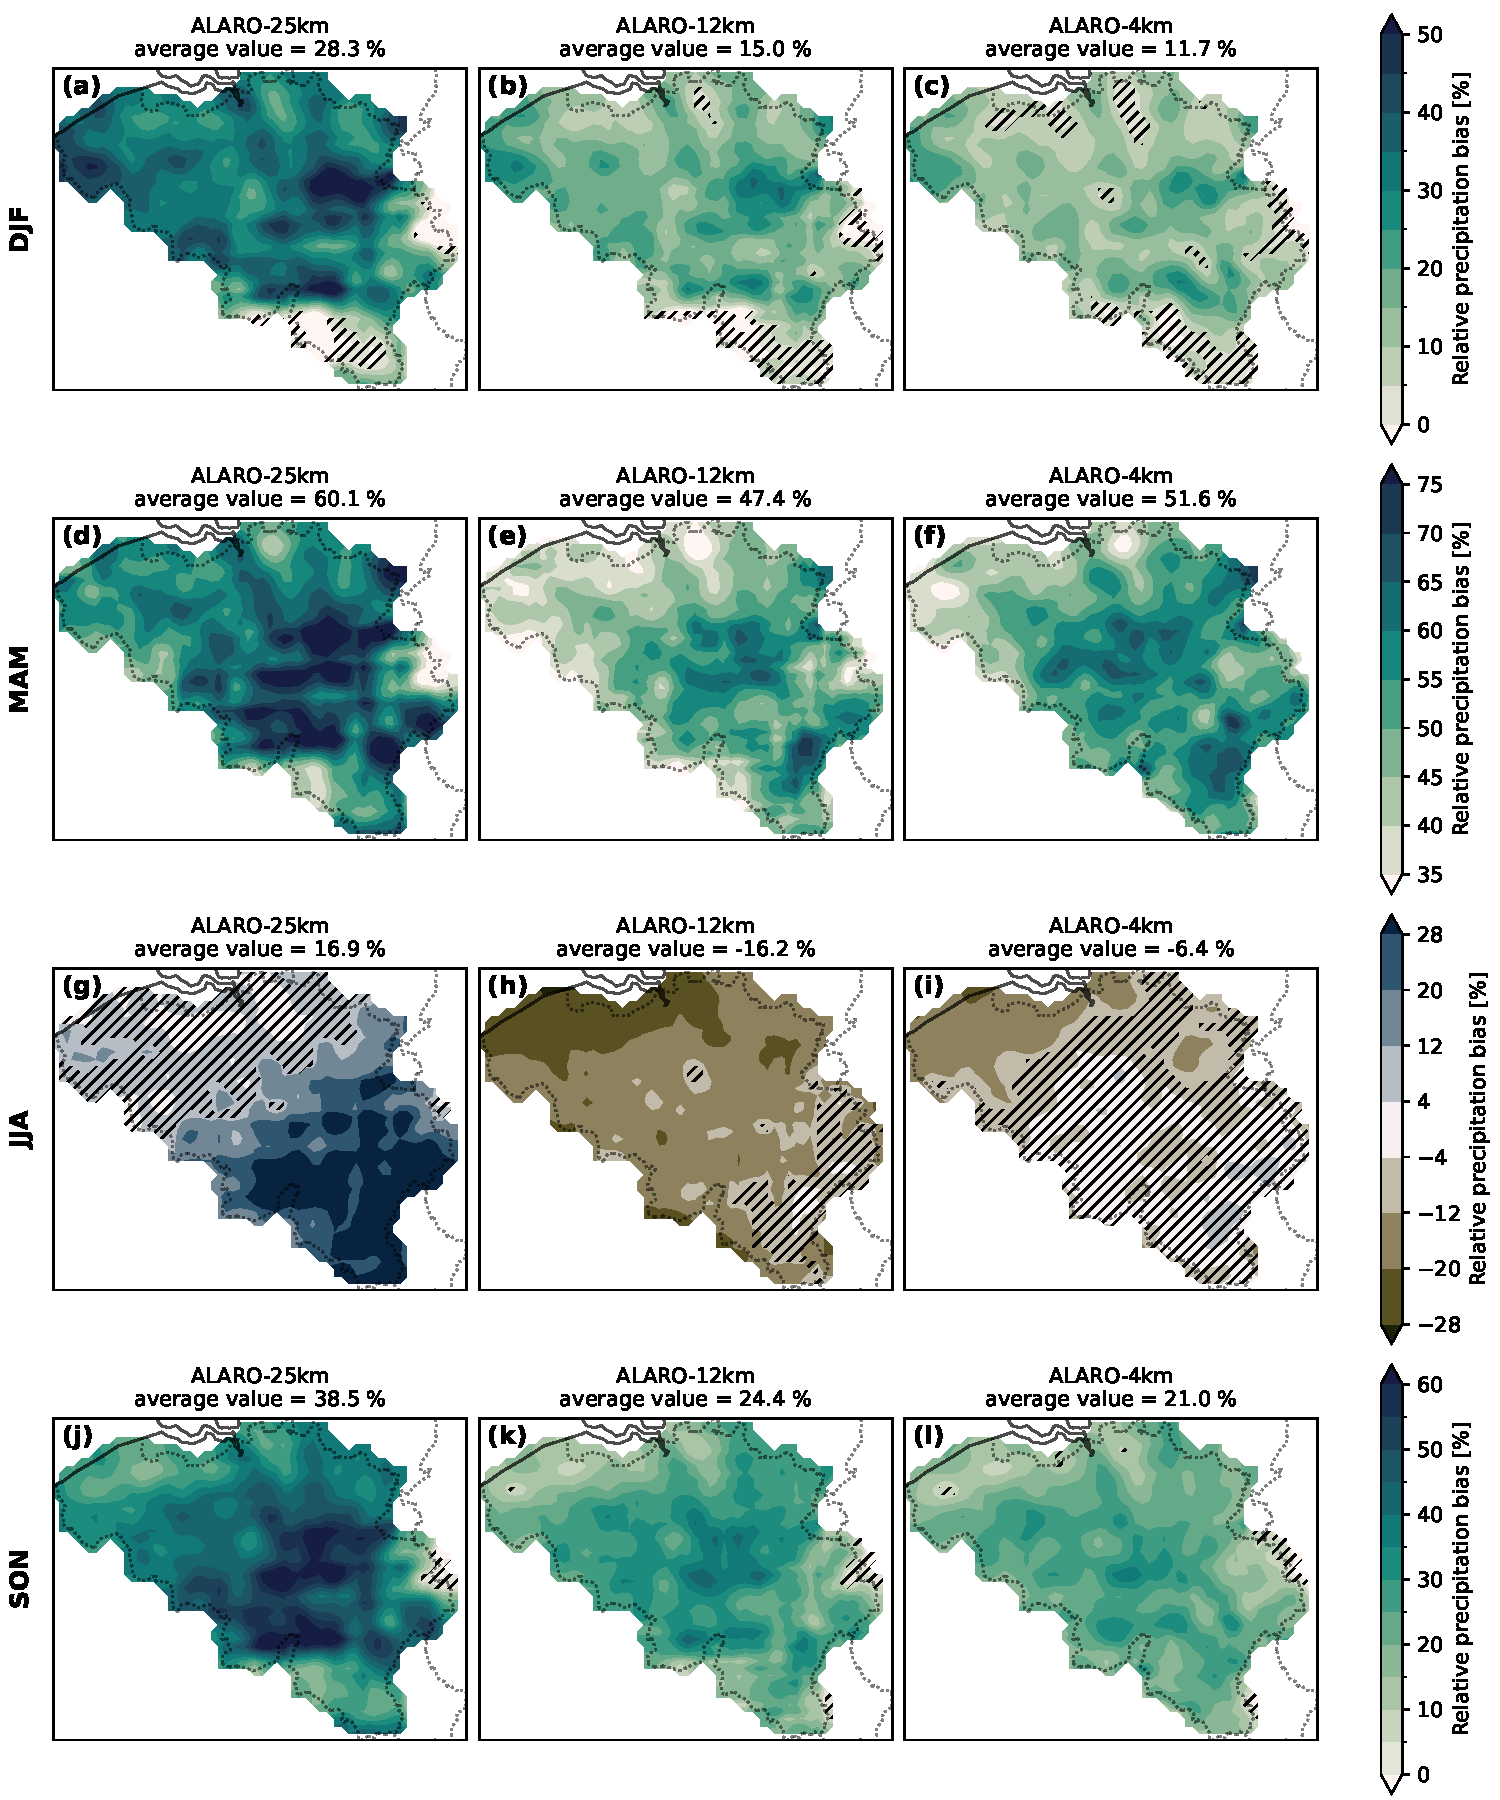
\includegraphics[width=12cm]{figures/figD2.pdf}
\caption{Bias in mean seasonal precipitation of each simulation (25 km, 12.5 km, and 4 km resolutions) with respect to the daily gridded observational CLIMATE-GRID dataset over Belgium.}
\label{fig:pr_bias_seasons}
\end{figure*}
\newpage
\subsection{Extreme precipitation}
\begin{figure*}[h!]
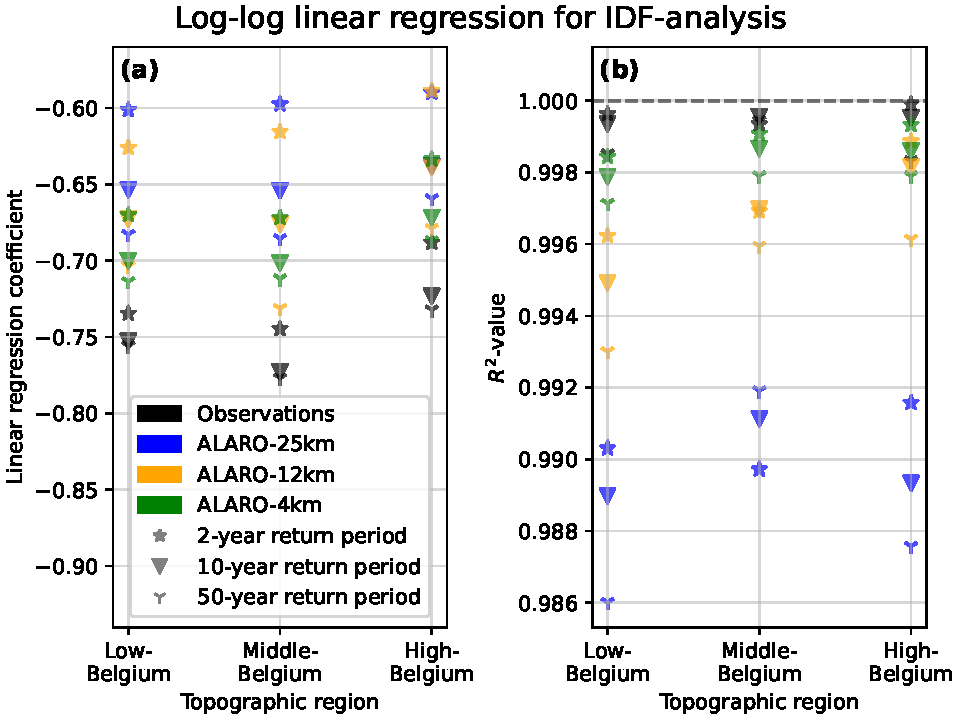
\includegraphics[width=\textwidth]{figures/figD3.pdf}
\caption{Log-log linear regression analysis of the return levels as a function of duration, performed for each dataset (observations and ALARO-simulations), topographic region, and return period separately. (left) The linear regression coefficients. (right) The $R^2$-values. The dashed line denotes a value of 1, which corresponds to a perfect fit.}
\label{fig:IDFs_linear}
\end{figure*}

% \subsection{}     %% Appendix A1, A2, etc.


\noappendix       %% use this to mark the end of the appendix section. Otherwise the figures might be numbered incorrectly (e.g. 10 instead of 1).

%% Regarding figures and tables in appendices, the following two options are possible depending on your general handling of figures and tables in the manuscript environment:

%% Option 1: If you sorted all figures and tables into the sections of the text, please also sort the appendix figures and appendix tables into the respective appendix sections.
%% They will be correctly named automatically.

%% Option 2: If you put all figures after the reference list, please insert appendix tables and figures after the normal tables and figures.
%% To rename them correctly to A1, A2, etc., please add the following commands in front of them:

% \appendixfigures  %% needs to be added in front of appendix figures

% \appendixtables   %% needs to be added in front of appendix tables

%% Please add \clearpage between each table and/or figure. Further guidelines on figures and tables can be found below.

\newpage

\codeavailability{The Python notebooks used for the analysis are available through \url{https://doi.org/10.5281/zenodo.15791682}~\citep{dewettinck_code_2025}.
The ALARO1-SFX code, along with all its related intellectual property rights, is owned by the members of the ACCORD consortium. Each member of this consortium can license the shared code to academic institutions of their home country for noncommercial research. 
Access to the codes of the ACCORD system can be obtained by contacting one of the member institutes mentioned in \citet{termonia_aladin_2018} or by submitting a request in the Contact link below the page of the ACCORD website (\url{https://www.umr-cnrm.fr/accord/}) and the access will be subject to signing a standardized ACCORD license agreement.}

\dataavailability{
The VMM rainfall observations over Flanders are available on \url{https://waterinfo.vlaanderen.be/}. The DHG rainfall observations may be requested from the Service public de Wallonie - Mobilité et Infrastructures, Direction de la Gestion hydrologique, PEREX, Rue Del’Grête, 22, 5020 NAMUR (Daussoulx). The IBGE data may be requested at the Bruxelles Environnement (\url{https://environnement.brussels}). The automatic weather station (AWS) rainfall observations from the Royal Meteorological Institute of Belgium are available on \url{https://opendata.meteo.be/download}. Annual maxima extracted from the HYDRO-network from the Royal Meteorological Institute of Belgium are available on \url{https://doi.org/10.5281/zenodo.4741177}. Further information about the CLIMATE-GRID dataset can be found on \url{https://opendata.meteo.be/geonetwork/srv/eng/catalog.search\#/metadata/RMI_DATASET_GRIDDEDOBS}, although the data are currently not yet publicly available.
The simulation data used in this study can be found on \url{https://doi.org/10.5281/zenodo.15296030}~\citep{dewettinck_data_2025}.
} %% use this section when having only data sets available

\authorcontribution{
SC and PT conceptualized the study. SC, PT, and WD acquired funding. WD conducted the investigation and performed the formal analysis. WD, KV and MVG were responsible for software implementation. HVdV, DD, RH, BVS, KVW, SC, and PT supervised the research. WD created the visualizations and prepared the original draft. All authors contributed to the review and editing of the manuscript and approved the final version.
} %% this section is mandatory

\competinginterests{The authors declare that they have no conflict of interest.} %% this section is mandatory even if you declare that no competing interests are present

\begin{acknowledgements}
The authors acknowledge the Flemish Supercomputer Center (VSC) for providing the computational resources and services used to perform the ALARO1-SFX regional climate simulations.
The authors also thank the Vlaamse Milieumaatschappij (VMM), the Direction de la Gestion Hydrologique (DGH) of SPW Mobilité et Infrastructures, and Brussels Environment for providing precipitation observations over Flanders, Wallonia, and Brussels, respectively.
Finally, we acknowledge the use of AI-assisted tools, which were used exclusively for language refinement and text rewriting. All scientific content was developed and validated by all authors.
\end{acknowledgements}

\financialsupport{This research has been supported by the Research Foundation – Flanders (FWO) (grant no. 1157523N). KV is supported by the Belgian Science Policy (BELSPO) under Contract B2/223/P1/CORDEXbeII. KVW is funded through Belspo grant FED-tWIN2021-prf024 - ARCHWAy. SC is supported by the BELSPO project FED-tWIN 2020-018\_AURA.}


%% REFERENCES

%% The reference list is compiled as follows:

% \begin{thebibliography}{}

% \bibitem[AUTHOR(YEAR)]{LABEL1}
% REFERENCE 1

% \bibitem[AUTHOR(YEAR)]{LABEL2}
% REFERENCE 2

% \end{thebibliography}

%% Since the Copernicus LaTeX package includes the BibTeX style file copernicus.bst,
%% authors experienced with BibTeX only have to include the following two lines:
%%
\bibliographystyle{copernicus}
\bibliography{references.bib} % Export from Zotero
%%
%% URLs and DOIs can be entered in your BibTeX file as:
%%
%% URL = {http://www.xyz.org/~jones/idx_g.htm}
%% DOI = {10.5194/xyz}


%% LITERATURE CITATIONS
%%
%% command                        & example result
%%~\citet{jones90}|               & Jones et al. (1990)
%%~\citep{jones90}|               & (Jones et al., 1990)
%%~\citep{jones90,jones93}|       & (Jones et al., 1990, 1993)
%%~\citep[p.~32]{jones90}|        & (Jones et al., 1990, p.~32)
%%~\citep[e.g.,][]{jones90}|      & (e.g., Jones et al., 1990)
%%~\citep[e.g.,][p.~32]{jones90}| & (e.g., Jones et al., 1990, p.~32)
%%~\citeauthor{jones90}|          & Jones et al.
%%~\citeyear{jones90}|            & 1990



%% FIGURES

%% When figures and tables are placed at the end of the MS (article in one-column style), please add \clearpage
%% between bibliography and first table and/or figure as well as between each table and/or figure.

% The figure files should be labelled correctly with Arabic numerals (e.g. fig01.jpg, fig02.png).


%% ONE-COLUMN FIGURES

%%f
%\begin{figure}[t]
%\includegraphics[width=8.3cm]{FILE NAME}
%\caption{TEXT}
%\end{figure}
%
%%% TWO-COLUMN FIGURES
%
%%f
%\begin{figure*}[t]
%\includegraphics[width=12cm]{FILE NAME}
%\caption{TEXT}
%\end{figure*}
%
%
%%% TABLES
%%%
%%% The different columns must be seperated with a & command and should
%%% end with \\ to identify the column brake.
%
%%% ONE-COLUMN TABLE
%
%%t
%\begin{table}[t]
%\caption{TEXT}
%\begin{tabular}{column = lcr}
%\tophline
%
%\middlehline
%
%\bottomhline
%\end{tabular}
%\belowtable{} % Table Footnotes
%\end{table}
%
%%% TWO-COLUMN TABLE
%
%%t
%\begin{table*}[t]
%\caption{TEXT}
%\begin{tabular}{column = lcr}
%\tophline
%
%\middlehline
%
%\bottomhline
%\end{tabular}
%\belowtable{} % Table Footnotes
%\end{table*}
%
%%% LANDSCAPE TABLE
%
%%t
%\begin{sidewaystable*}[t]
%\caption{TEXT}
%\begin{tabular}{column = lcr}
%\tophline
%
%\middlehline
%
%\bottomhline
%\end{tabular}
%\belowtable{} % Table Footnotes
%\end{sidewaystable*}
%
%
%%% MATHEMATICAL EXPRESSIONS
%
%%% All papers typeset by Copernicus Publications follow the math typesetting regulations
%%% given by the IUPAC Green Book (IUPAC: Quantities, Units and Symbols in Physical Chemistry,
%%% 2nd Edn., Blackwell Science, available at: http://old.iupac.org/publications/books/gbook/green_book_2ed.pdf, 1993).
%%%
%%% Physical quantities/variables are typeset in italic font (t for time, T for Temperature)
%%% Indices which are not defined are typeset in italic font (x, y, z, a, b, c)
%%% Items/objects which are defined are typeset in roman font (Car A, Car B)
%%% Descriptions/specifications which are defined by itself are typeset in roman font (abs, rel, ref, tot, net, ice)
%%% Abbreviations from 2 letters are typeset in roman font (RH, LAI)
%%% Vectors are identified in bold italic font using \vec{x}
%%% Matrices are identified in bold roman font
%%% Multiplication signs are typeset using the LaTeX commands \times (for vector products, grids, and exponential notations) or \cdot
%%% The character * should not be applied as mutliplication sign
%
%
%%% EQUATIONS
%
%%% Single-row equation
%
%\begin{equation}
%
%\end{equation}
%
%%% Multiline equation
%
%\begin{align}
%& 3 + 5 = 8\\
%& 3 + 5 = 8\\
%& 3 + 5 = 8
%\end{align}
%
%
%%% MATRICES
%
%\begin{matrix}
%x & y & z\\
%x & y & z\\
%x & y & z\\
%\end{matrix}
%
%
%%% ALGORITHM
%
%\begin{algorithm}
%\caption{...}
%\label{a1}
%\begin{algorithmic}
%...
%\end{algorithmic}
%\end{algorithm}
%
%
%%% CHEMICAL FORMULAS AND REACTIONS
%
%%% For formulas embedded in the text, please use \chem{}
%
%%% The reaction environment creates labels including the letter R, i.e. (R1), (R2), etc.
%
%\begin{reaction}
%%% \rightarrow should be used for normal (one-way) chemical reactions
%%% \rightleftharpoons should be used for equilibria
%%% \leftrightarrow should be used for resonance structures
%\end{reaction}
%
%
%%% PHYSICAL UNITS
%%%
%%% Please use \unit{} and apply the exponential notation


\end{document}
